\documentclass[titlepage]{article}

\usepackage[margin=1.5in]{geometry}
\usepackage{graphicx}
\usepackage{hyperref}
\usepackage{float}
\usepackage{placeins}
\usepackage{amsmath}
\usepackage[noabbrev,nameinlink]{cleveref}

\title{COMS 4444: Project 3, Group 8}
\author{Jeffrey Tao, Martin Ristovski, Vikram Rajan}
\date{November 2022}

\begin{document}

\maketitle

\tableofcontents

\pagebreak

\section{Introduction}

A Magical Code is the third project of COMS W4444 taught by Professor Kenneth Ross in the Fall 2022 semester at Columbia University. In class, we discussed several different ideas on how to most accurately and robustly encode messages with a deck of cards. Our group consists of 3 members: Jeffrey Tao, Martin Ristovski, and Vikram Rajan. In this report, we will define the specifications of the problem, discuss our initial thoughts and ideas, and then detail the final solution we implemented. 

\subsection{Problem Specification}

The premise of A Magical Code is to encode a secret message you want to send to someone, but only using a standard deck of playing cards. As there are only 52 cards, there is a limit on the length of message we can send, but our job was to see just how long of a message we could send and still send meaningful information. Another limiting factor we faced was the ability of our decks to withstand random shuffling. In the war analogy this problem was presented to us as, this was to circumvent suspicious guards by showing them there could not possibly be a message contained in the deck of cards, as you can randomly shuffle the top cards many times. Given these constraints, we have to be able to encode and decode a message in the deck, but also be able to label random decks as NULL. 

The goal is to be able to send as long as a message as possible given the constraints. Another option is to recover a partial message, as this would be more advantageous than recovering gibberish. These partial matches have to be specifically indicated, thus requiring some bits to do so. It also must be an exact prefix match, so it cannot randomly splice together parts of the original message, as that might not mean anything to the receiver. 

\section{Initial Implementation}

\subsection{Separating Messages, Bits, and Cards}
As discussed in class, we implemented separate schemes for encoding string messages to bits and for encoding bits to cards. This allowed us to work on these parts independently and optimize them separately. As the project wore on, this strategy bore fruit as it enabled us to write many different message-to-bits encoders for the different tournament message domains.

\subsection{Message-to-bits: Huffman Coding}
Our initial intuition for encoding messages to bits was to exploit the disparity between how frequently letters occur in the English language. To do this, we found a frequency distribution of the letters of the alphabet in English and used that to generate a Huffman coding. Huffman coding works on the principle that more common characters should have shorter encodings, and less common characters can have longer encodings. Huffman coding is also a \textit{prefix encoding}, meaning that decoding requires no backtracking, as each character has a unique prefix such that decoding is unambiguous. When a character is matched, it is safe to emit that character.

\subsection{Bits-to-cards: Card Index Encoding}
Now that we had a mapping from characters to bits, we needed a mapping from bits to cards. To do this, we take our bitstring and the number $c$ cards we want to encode it in. Assuming the integer value of the binary string is less than $c!$, we divide that up into $c$ bins of size $(c-1)!$. We proceed bit-by-bit, choosing indexes according to the ordering of the remaining un-used cards, as cards can not be reused. Finally, the message encoded in $c$ cards goes at the bottom of the deck, as cards towards the bottom are more resistant to shuffles. The top of the deck is padded with the remaining $52-c$ cards in order.

Decoding requires a known value of $c$ (discussed below in \cref{metadata}). Given $c$, we first filter out all card with values $> c$, as they are irrelevant and may have been mixed into the bottom cards due to shuffles. We recover the input bit string by performing the reverse indexing process: for each place value, we know the bin width, and can find the index of the bin via the index of the current card in the ordering of all currently remaining cards. After recovering the bit string, we can try to decode the message.

\subsection{Metadata} \label{metadata}
We store metadata at the end of our message, where it is most durable. Our initial message metadata consisted of a length byte and a checksum byte. As the project went on, we changed our metadata logic to make these fields variable in length, removed the length byte, and added bits to denote different string-to-bits message encodings.

We do not actually know the value of $c$ used to encode bits in the deck. As such, in order to recover the bit string, we need to try every possible value of $c$. However, without some protections, we could recover any bit string from any deck, making recovering the original mesasge impossible. As such, we introduced a checksum to the bitstring. The checksum is computed by taking some function over the bits of the message and appending the output bits to the message. As long as the checksum is of a known length, we can recover messages by trying many values of $c$, taking the last bits as the message checksum, re-computing the checksum function over the remaining bits, and seeing if they match. If they do match, we have high confidence that this is the message that we intended to recover. If they do not match, we are guaranteed that this is not the message we wanted to recover.

Furthermore, due to our bits-to-cards integer encoding scheme, we found that leading 0's would be dropped when decoding the bit string from cards. As such, we elected to add a length byte to the message metadata. A better solution to this problem is discussed in \cref{no_length_byte}.

\begin{figure}
    \centering
    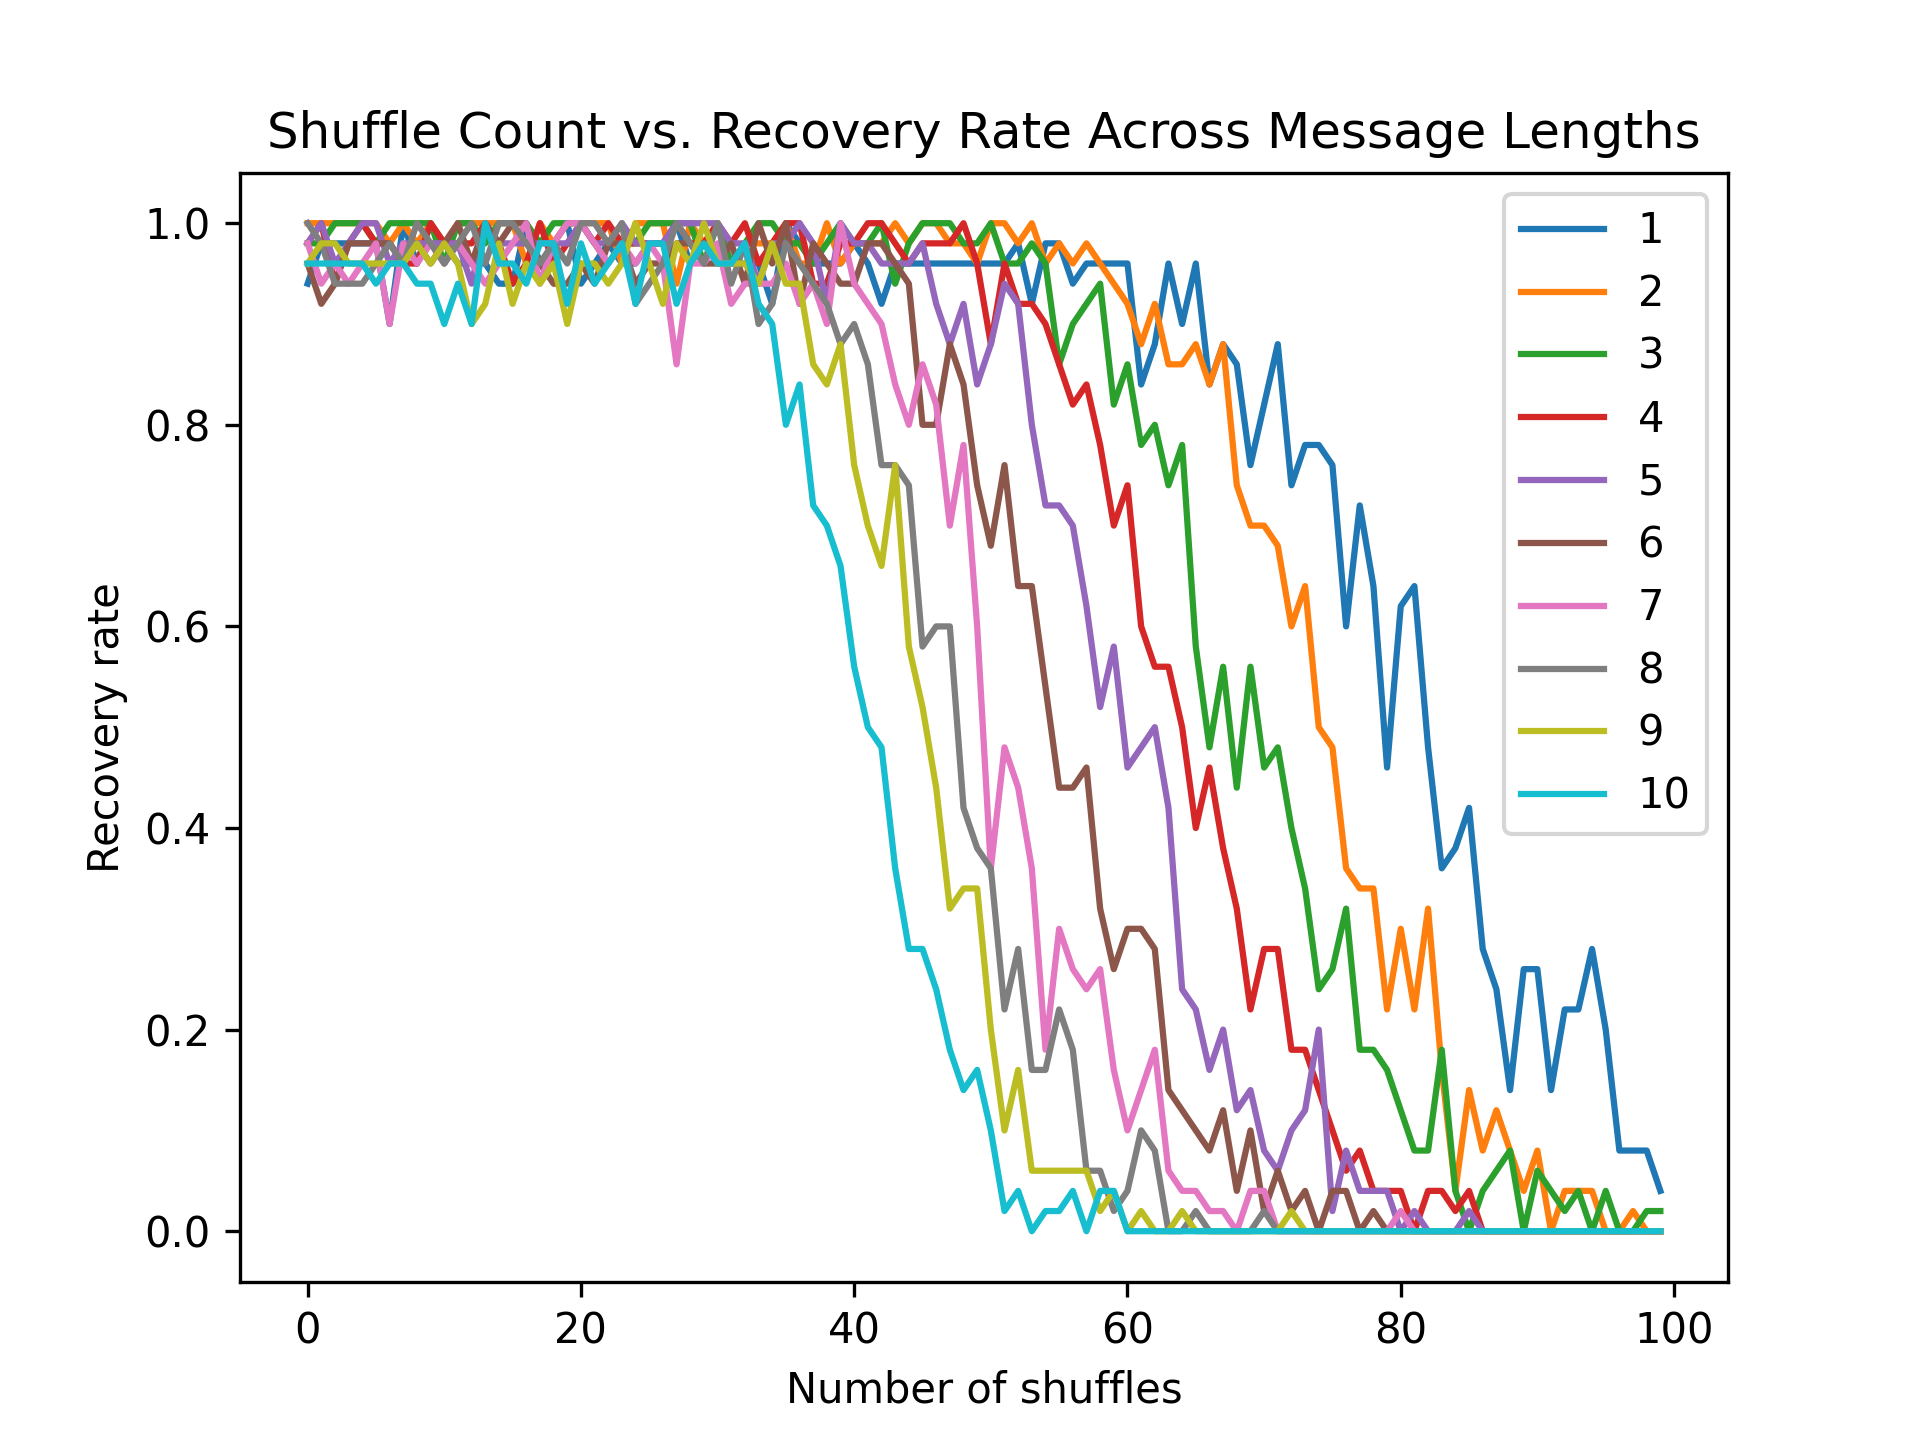
\includegraphics[width=\textwidth]{figures/early_agent.png}
    \caption{Our initial agent's performance on sequences of lowercase letters drawn uniformly randomly. The vertical axis shows recovery rate, i.e. the proportion of messages that are exactly recovered. Number of shuffles increases along the horizontal axis. Each color encodes the length of the message: longer messages tend to be harder to recover, while shorter messages survive more shuffles.}
    \label{fig:early_agent}
\end{figure}

Our early performance was already quite promising, shown in \Cref{fig:early_agent}.

\FloatBarrier

\section{Improvements}

While our solution performed well within this limited message domain, to do well on the tournament there were a number of extensions that we'd need to make. 

\subsection{Better Checksum}
One of the easier adjustments we made was in order to reduce the rate of checksum collision to further avoid false positives. The purpose of the checksum is to prevent the decoder from deciphering random decks as meaningful messages; however, with the random shuffles, there would be times where the checksum would pass for an invalid message. With an 8-bit checksum, we expected this false positive rate to be 1 out of 256, but the rate we recorded was significantly higher. To accomplish this, we increased the length of our checksum from 8 to 10 bits, which gave us a 4x reduction in the false positive rate.

The variable-length checksum function we implemented took advantage of a cryptographic hashing function called sha256 from Python's hashlib library. This takes in the bitstring, creates a hash as a long hexstring, which we then convert to binary and take the lowest x bits. Having a configurable checksum length also proved to be a boon later in the project as it allowed us to experiment freely with checksum lengths to tweak messsage recovery performance.

\begin{figure}
\makebox[\textwidth][c]{
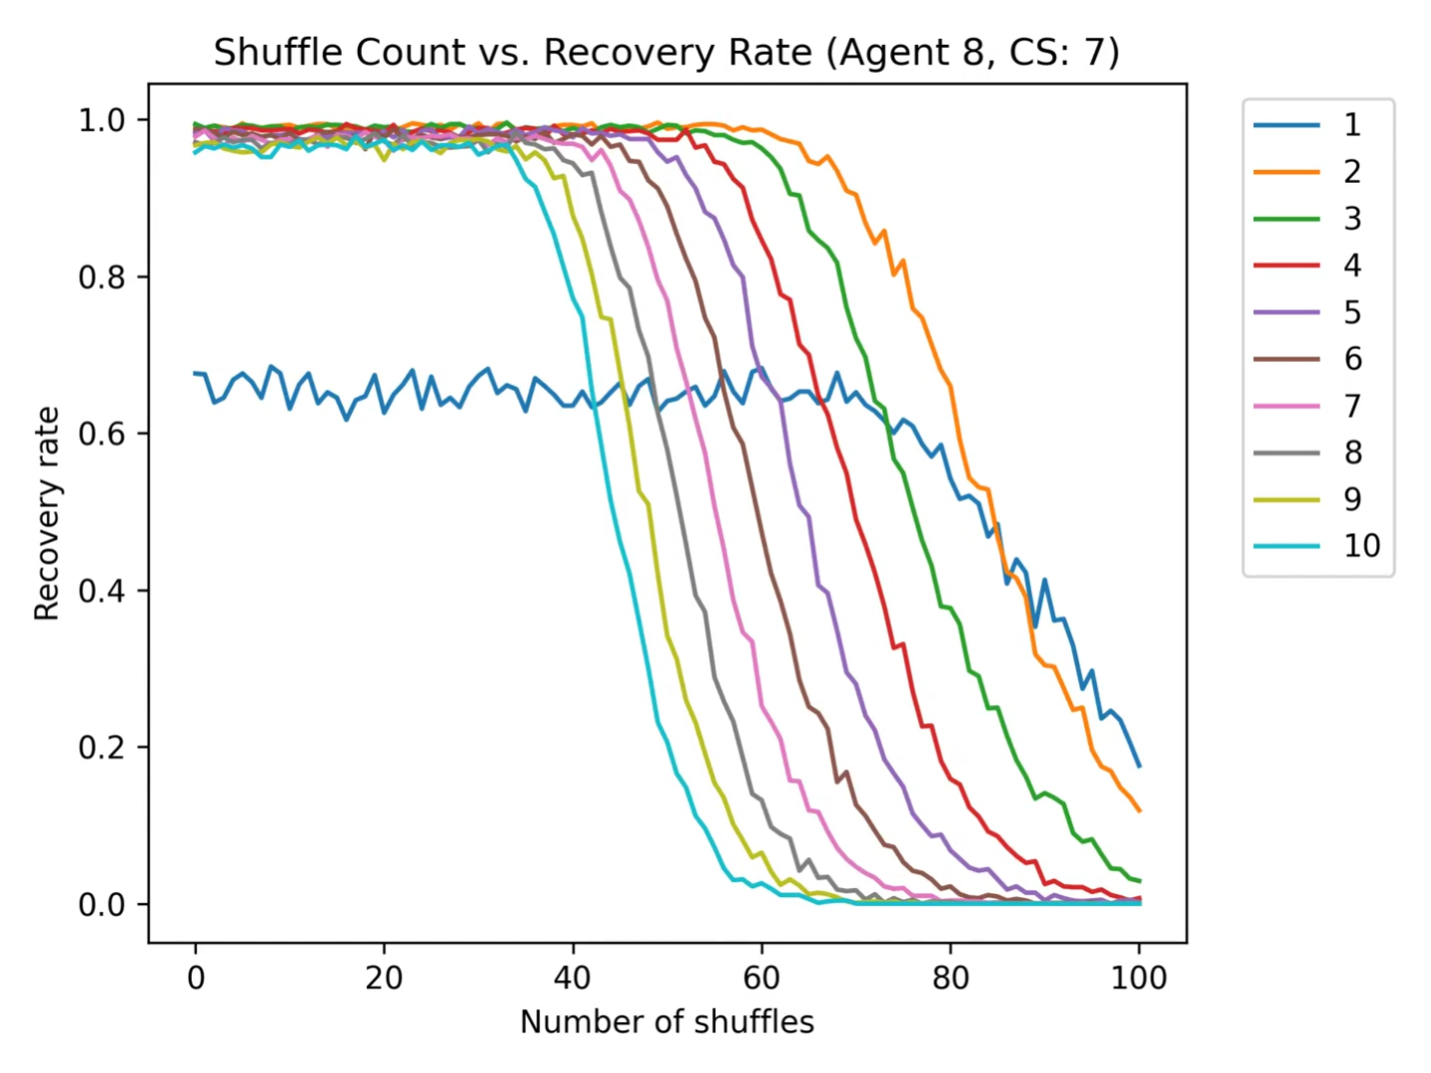
\includegraphics[width=0.45\paperwidth]{figures/checksum_7.png}
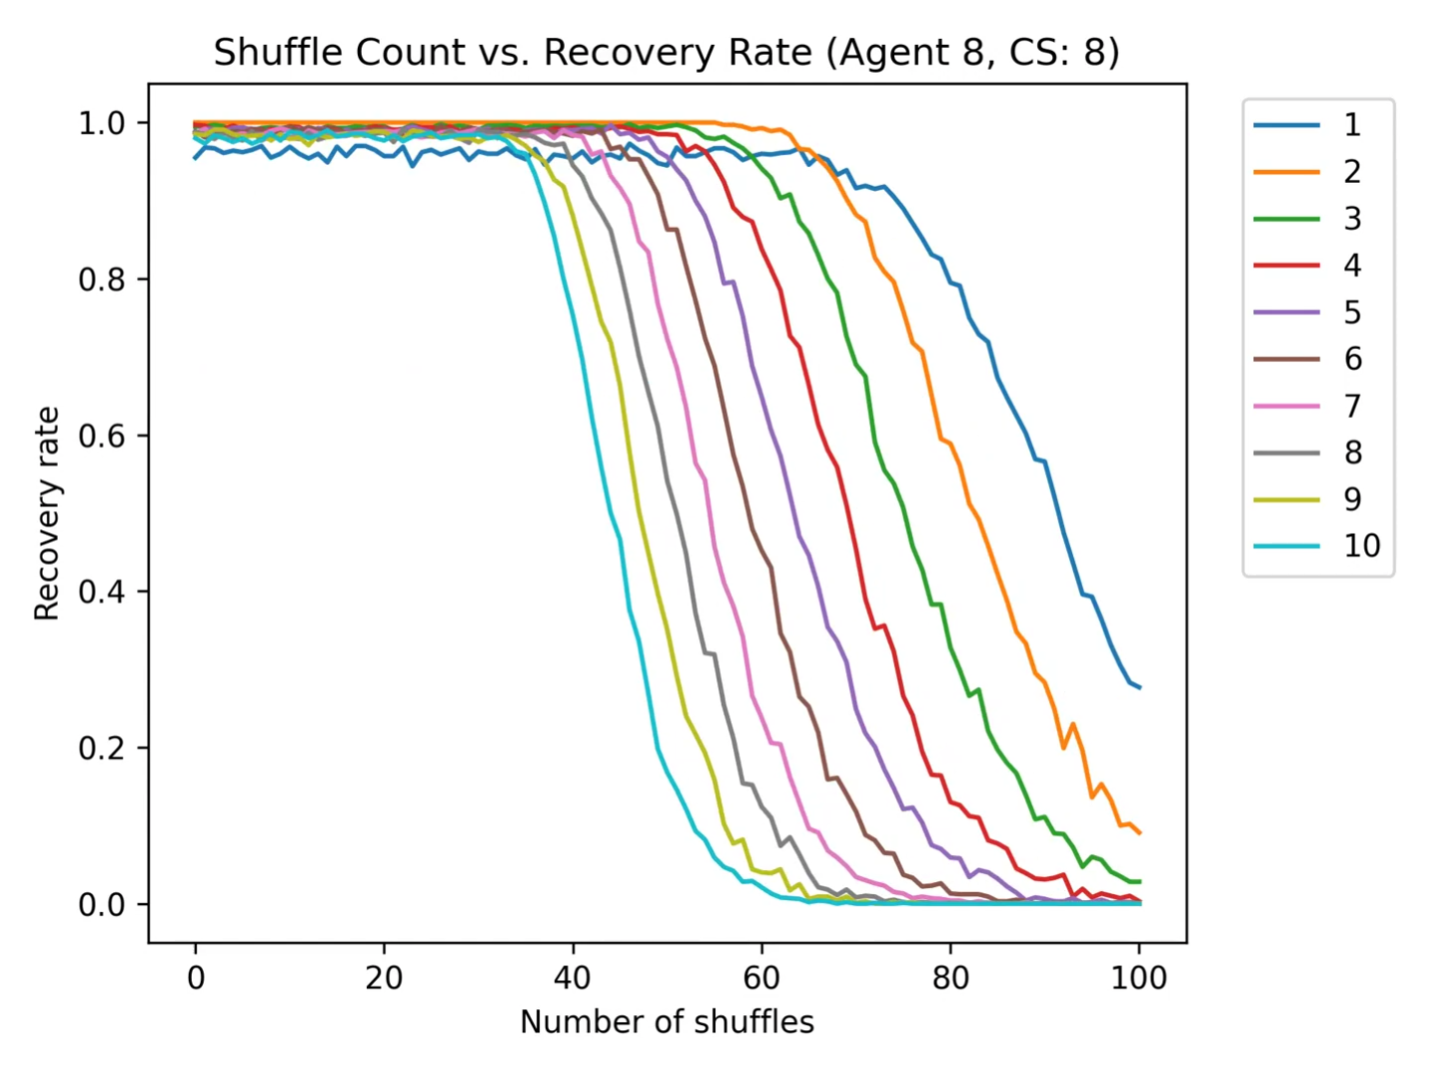
\includegraphics[width=0.45\paperwidth]{figures/checksum_8.png}
}
\makebox[\textwidth][c]{
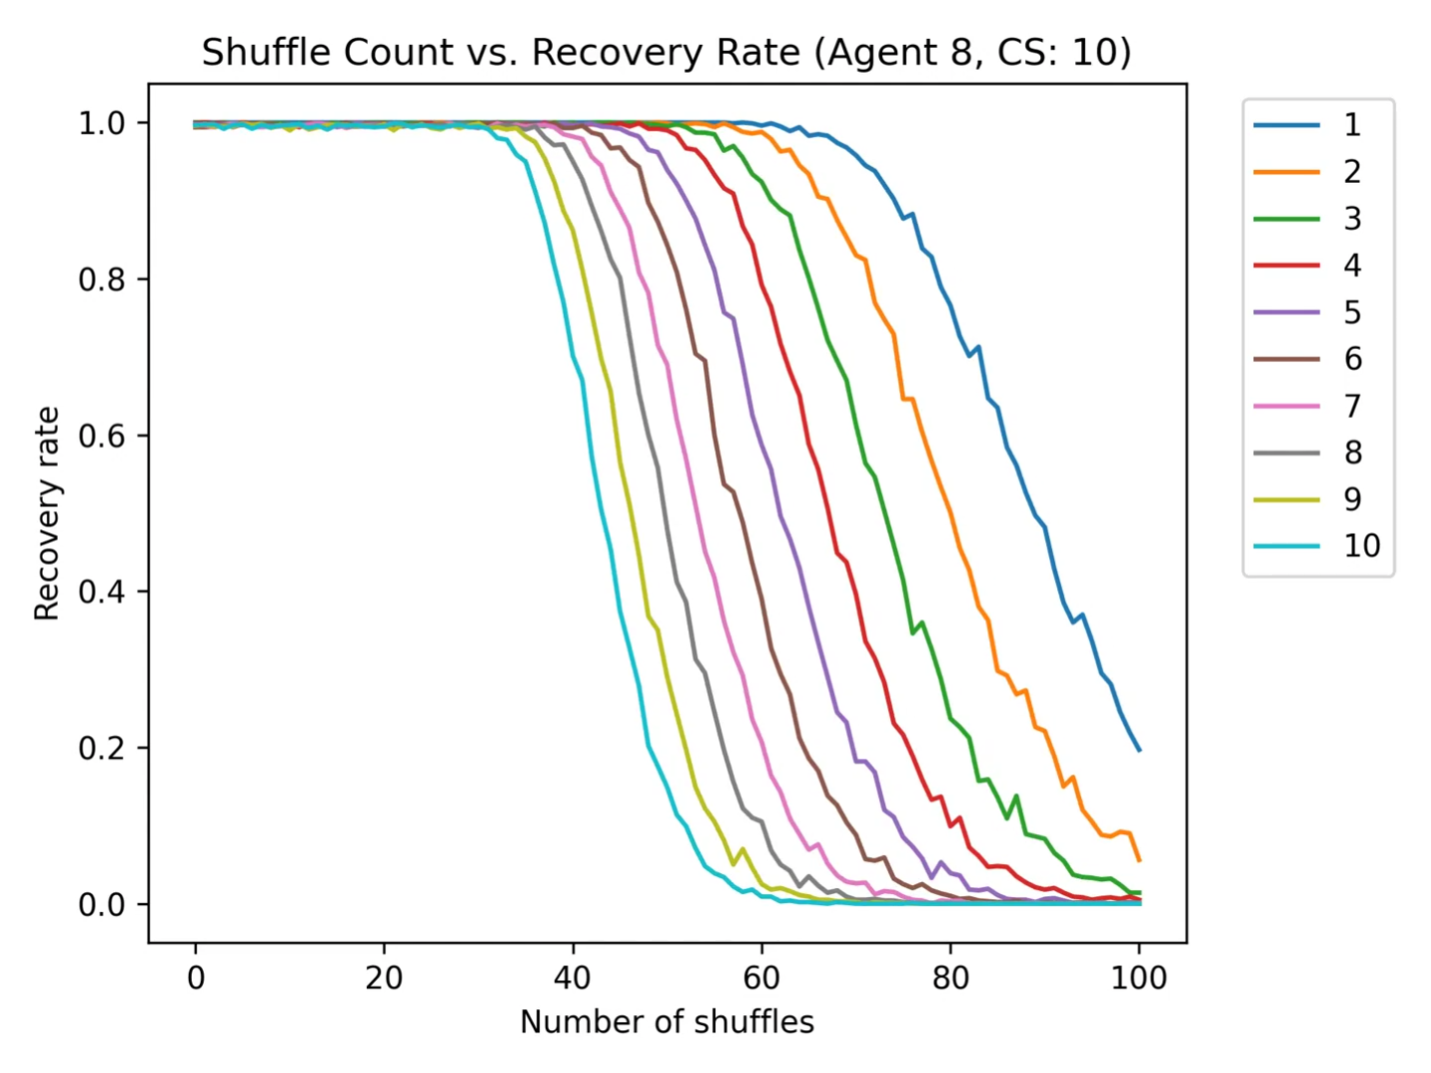
\includegraphics[width=0.45\paperwidth]{figures/checksum_10.png}
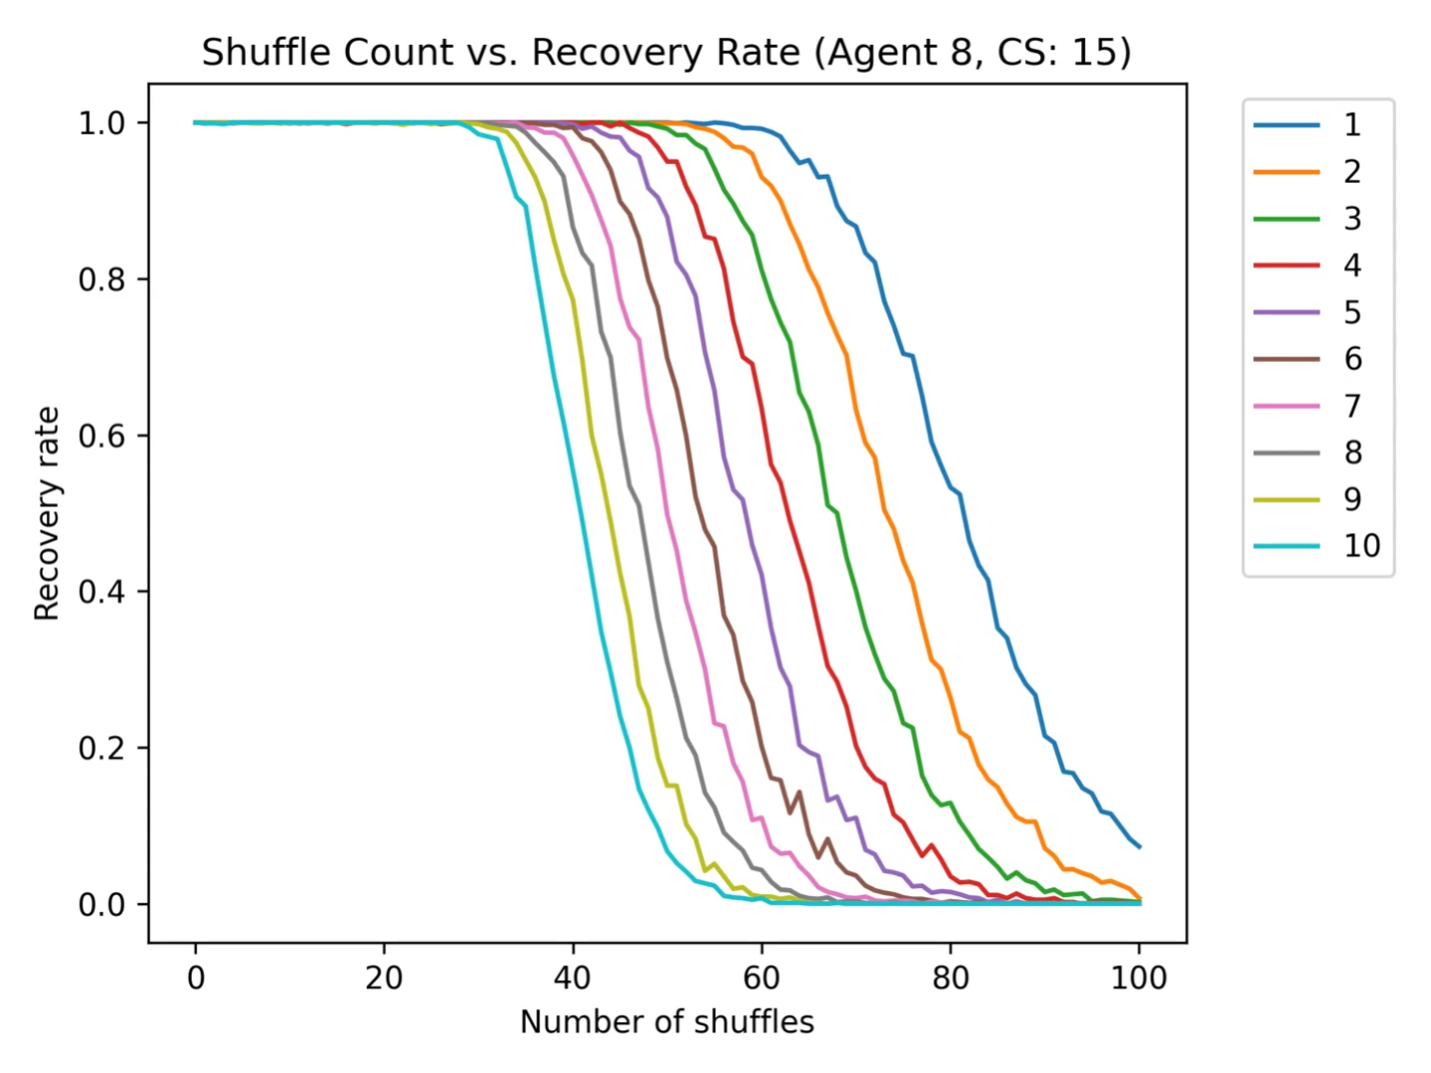
\includegraphics[width=0.45\paperwidth]{figures/checksum_15.png}
}
\caption{Comparison of message recovery performance for checksums of length 7, 8, 10, and 15 bits. Longer checksums rapidly improve performance up to approximately 10 bits by reducing the probability of message decode collisions, after which longer checksums diminish performance by making the metadata section longer.}
\end{figure}

\subsection{Multiple Domains}
Then, we added support for multiple message domains. Implementing multiple domains allowed us to use a more efficient encoding scheme for each domain, which in turn decreased the length of our message and made it more resistant to shuffles. However, we also had to dedicate 3 bits of our bitstring to let the decoder know which scheme was used to encode the message. In our testing, this was a worthwhile tradeoff. We added a number of character-based encoding schemes, which also used Huffman coding but with a different set of characters and thus a different frequency distribution. In particular, we added a domain containing only numbers, a domain containing charcters typically found in English writing (uppercase and lowercase letters, numbers, space, and a few punctuation marks), and a domain containing all printable ASCII characters, which we used as a fallback of sorts, since it is able to encode any message at the cost of efficiency.

\subsection{Dictionary-based Encoding Schemes}
We further extended our multiple domain approach by implementing word-based encoding schemes. These would map words to integers that referrenced each word's position in a dictionary, allowing the decoder to simply look up each word. This meant that if all words in a message are present in our dictionary, we could encode much longer messages than if we were to use a character-based encoding scheme. The dictionaries we initially included were one of a large number of words in the English language, one of names of people, and one of names of places.

\subsection{Removing the Length Byte} \label{no_length_byte}
In our initial scheme, we stored a length byte in the message metadata. For messages with leading 0's (i.e. the message has a prefix consisting of some number of 0's), it is impossible to recover the leading 0's using our bits-to-cards indexed encoding scheme, as the reverse cards-to-bits function returns an integer value. As such, any leading 0's would be lost, so we added message length to the metadata so that we could manually pad the recovered message with 0's to decode.

\begin{figure}
    \centering
    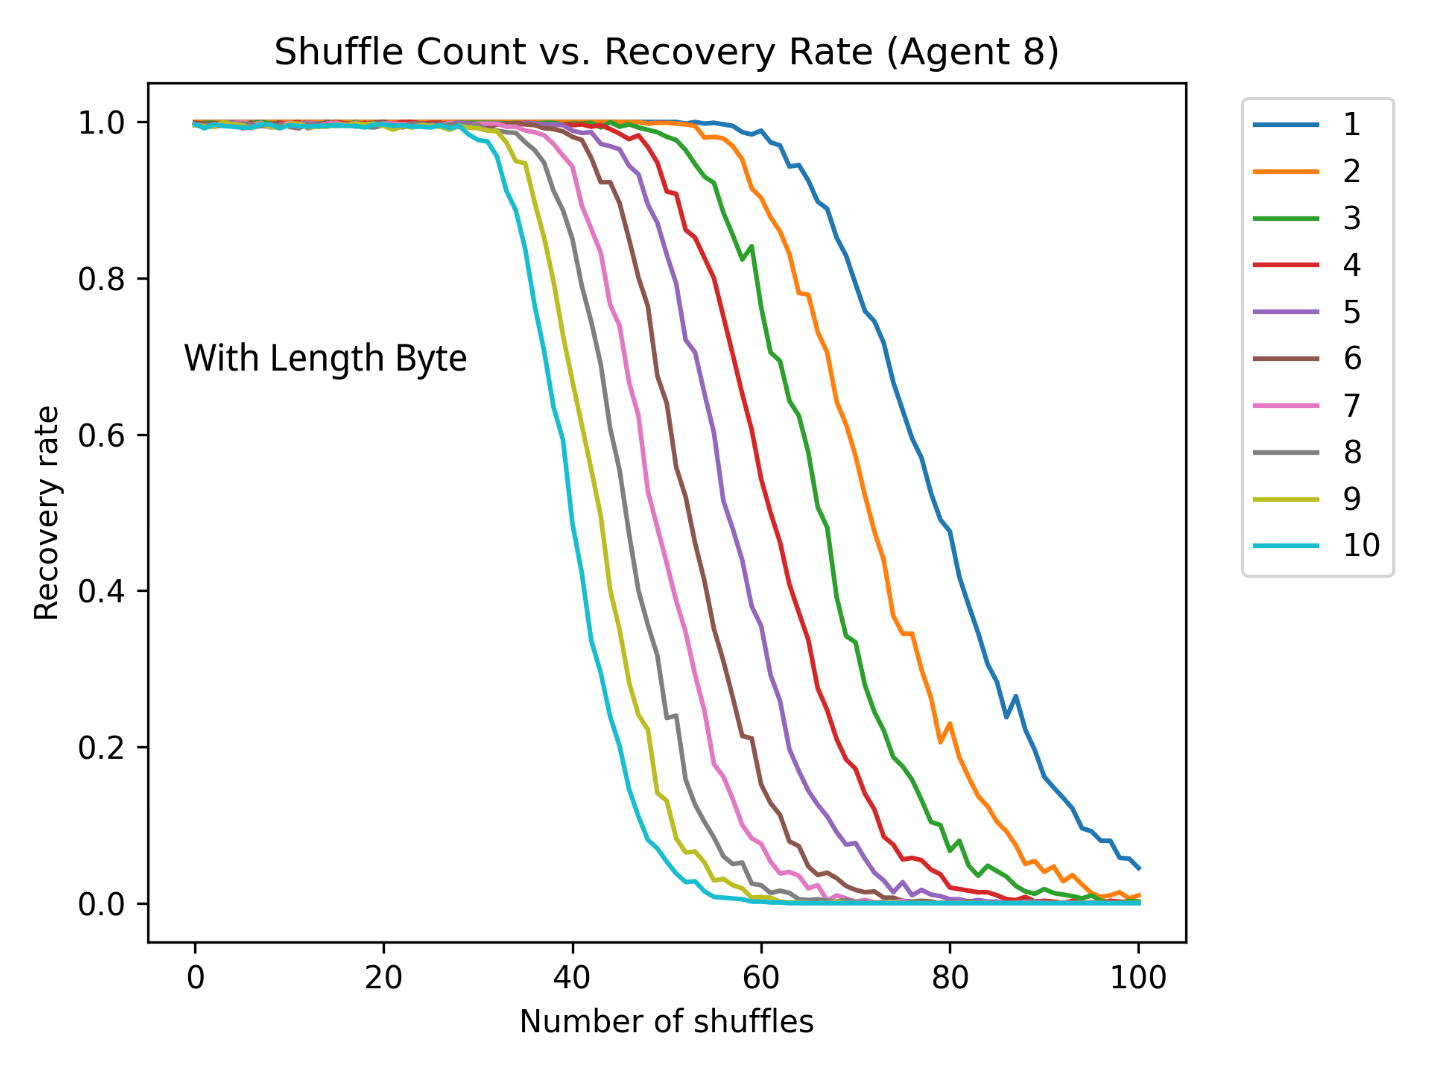
\includegraphics[width=0.9\textwidth]{figures/length_byte.png}
    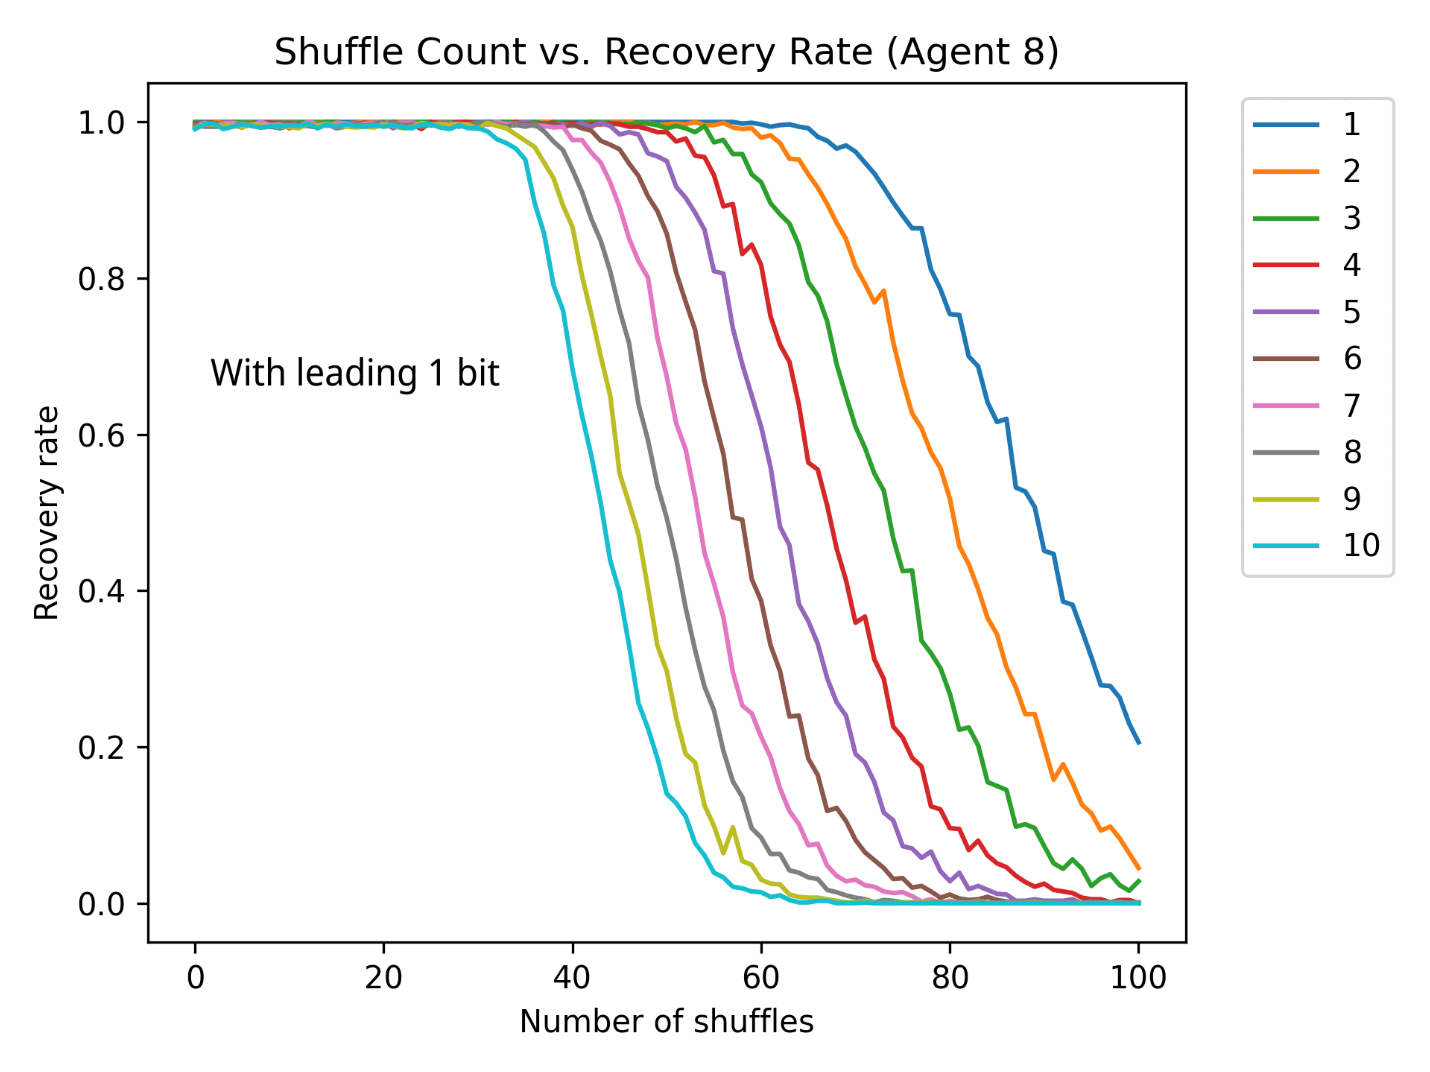
\includegraphics[width=0.9\textwidth]{figures/leading_1.png}
    \caption{Above: recovery curves on the domain of random lowercase letters for our agent using the length byte. Below: recovery curves on the same domain for our agent using the leading 1 bit. Removing 7 bits from the metadata pushes all of the curves towards the right, meaning that more messages survive a higher number of shuffles.}
    \label{fig:no_length_byte}
\end{figure}

Group 3 suggested that we could prepend a 1 bit to the message to preserve leading 0's, and remove the 1 bit before decoding. This allowed us to remove the length byte entirely and save 7 bits of metadata, which improved our agent's performance slightly. This is visualized in \Cref{fig:no_length_byte}.

\FloatBarrier

\section{Eight Tournament Domains} \label{domains}

On November 1, 2022, the class collectively decided to limit the types of messages to ones belonging to 8 domains, one proposed by each group, and each defined by a generator function. Our initial multi-domain apporach allowed us to easily adapt to this part of the tournament specifications, as we were able to build specific encoding schemes for each domain.

The domain we proposed consists of messages containing names of people and places separated by spaces, as we thought it would be a reasonable proposition that could realistically be used by a spy agency.

To achieve the best possible message recovery rates given our bit-to-card encoding scheme, we wrote custom message-to-bit encoders for each proposed tournament domain by reverse engineering the corresponding generator code. Below, we detail the message domains and our custom encoders.

We use a few generic techniques, referred to below, to encode messages in each of the following domains. In general, we strip away any constant, predictable syntax (field delimeters, message prefix/suffix, e.g. the leading @ sign in Group 3's password domain) and only encode the variable part.
\begin{enumerate}
    \item\textbf{Dictionary indexing} For message domains that draw from a word list, we load the word list and assign numbers to each word in the list. This allows words to be referred to efficiently by their index instead of encoding the actual letter sequence.
    \item\textbf{Constant widths} For messages with highly regular structure but variable length, we can break the message into tokens and encode each token in a constant number of bits $b$. This way, we can decode variable-length messages with no additional information by reading each $b$ bits from the start to the end.
    \item\textbf{Named known-width fields} For messages with highly regular structure that can be broken into separately encoded parts (henceforth, fields), we can choose a well-known ordering of fields for the domain and encode the message as the concatenation of the fields in the well-known ordering. To decode, we read the number of bits corresponding to the width of each successive field and reassemble the message.
    \item\textbf{Prefix identification} For messages consisting of concatenations of fixed-width parts, we use the leading bits to identify the token type, which gives the corresponding type length. Thus, we decode the message as a stream, first reading the type $t$ from the encoding prefix, then the next $b_t$ bits, then the next encoding prefix.
\end{enumerate}

\paragraph{Group 1: Random Characters}
Group 1's generator produces messages of arbitrary length consisting of lowercase letters, digits, space, and period drawn uniformly randomly. As such, we use \textbf{constant width} sequences mapping bits to indexes in an ordered list of all possible characters (6 bits per character). When decoding, we read each 6 bits and output the corresponding character whose index in the domain is given by the corresponding numeric value.

\paragraph{Group 2: Flights}
Group 2's generator produces messages consisting of 3-letter airport codes, 4-character reservation IDs, and 8-digit dates, representing a particular flight that an agent should fly on. Our agent encodes this via 5 \textbf{named known-width fields} fields: airport, reservation, month, day, year.

We have the list of all airport names, so we use \textbf{dictionary indexing} to encode them. Reservation codes are length 4 with a known alphabet of uppercase letters and digits, so we use $\left\lceil log_2(36)\right\rceil = 6$ bits to encode each character.

We encode month, day, and year separately as the number of possible dates is much smaller than the corresponding range of numbers, i.e. 01312023 is a valid date, but 14999999 is not. The highest expressible date, $\left\lceil{log_2(12282025)}\right\rceil = 24$, whereas $\left\lceil{log_2(12)}\right\rceil + \left\lceil{log_2(28)}\right\rceil + \left\lceil{log_2(4)}\right\rceil = 11$, so we save 13 bits this way.

\paragraph{Group 3: Passwords} Group 3's generator produces passwords consisting of digits and words. We do not know what order digits and words appear due to a shuffle operation in the generator: sometimes, two words will be adjacent, sometimes an unknown number of consecutive digits. As such, we use a \textbf{prefix identification} encoding, as described above. A 0 prefix denotes a single digit while a 1 prefix denotes an indexed word. Since the number of consecutive digits is unknown, we encode each digit separately to avoid encoding digit sequence length. Words are encoding with \textbf{dictionary indexing}. We strip off the initial @ sign and add it back when decoding.

\paragraph{Group 4: Coordinates} Group 4's generator produces latitude/longitude pairs. Degree values always have exactly 4 decimal places, so we can store all degree values using 7-digit decimal numbers (when decoding, leading 0's in the integer part are ignored). To store the full coordinate, we use \textbf{named known-width fields} for latitude degree, latitude N/S bit, longitude degree, longitude E/W bit. When decoding, we add back formatting (spaces, separating comma).

\paragraph{Group 5: Addresses} Group 5's generator produces random addresses. Street names and suffixes are drawn randomly from dictionaries, while address number can be 1 to 4 digits, possibly with leading 0's. To handle leading 0's, we also store the number length, and pad with 0's if necessary. We use \textbf{named known-width fields} to store number, number length, street name, street suffix, and trailing space bit. Street name and suffix are encoded using \textbf{dictionary indexing}. We found that Group 5's generator had a bug causing it to add a trailing space to all generated addresses except for the last one, so we store an extra bit to denote the presence of a trailing space.

\paragraph{Group 6: n-grams} Group 6's generator produces phrases of $n$ words from a corpus of n-grams derived from recent news articles. As this generator effectively generates ``words'' from a set of 10 dictionaries, we use \textbf{named known-width fields} to store $n$ and a \textbf{dictionary index} into the corresponding $n$-dictionary. We found a slight bug with the n-gram lists in which they sometimes contained $(n-1)$-grams. To compensate, we also search all dictionaries $n' \ge n$ to try to find the corresponding $n$ and index.

\paragraph{Group 7: Words} Group 6's generator produces sequences of space-separated words drawn uniformly randomly from a dictionary. As such, we use \textbf{constant width} fields corresponding to \textbf{dictionary indexes}. We found that some of the bugged $(n-1)$-grams from Group 6 collided with words in Group 7's dictionary. As such, the encoder for Group 7's generator rejects messages with trailing spaces so that they can instead be encoded by the n-gram encoder.

\paragraph{Group 8: Names \& Places} As mentioned earlier, we chose to generate messages with words randomly drawn from dictionaries of names and places. Thus, we use a \textbf{prefix identification} scheme in which a preceding 0 bit denotes a name with a preceding 1 bit denotes a place. The following bits are extracted as \textbf{dictionary indexes}. We realized later that the savings from using this scheme are very marginal: there are 18240 names and 10197 places, which differ by 1 bit in length when encoded. The savings in encoding in this way (vs. combining the dictionaries) would be more substantial for a larger disparity in the dictionary lengths.

\section{Tournament Performance}
In the tournament, each generator was used to generate 3 ``batches'' of messages, each containing a certain number of messages. The message content in a batch was held constant as the number of shuffles $n$ was varied. Batches and shuffle permutations were held constant across all agents to get as close of a comparison between agents as possible.

The analyses below were performed by coalescing all available results for each (agent, domain) pair, meaning that batches were treated as being all one batch. One caveat is that not all batches were run on all agents due to timeouts. The total number of results per-group per-domain are visualized in \Cref{fig:totals}. This means that in the per-domain analyses below, results for groups 1, 5, and 7 are backed by the most datapoints; with groups 2, 3, and 4 having an order of magnitude fewer datapoints; and groups 6 and 7 having fewer still. In the analyses below, we use average recovery rate, i.e. for all datapoints $D_i$:

\begin{figure}[ht]
    \makebox[\textwidth][c]{
        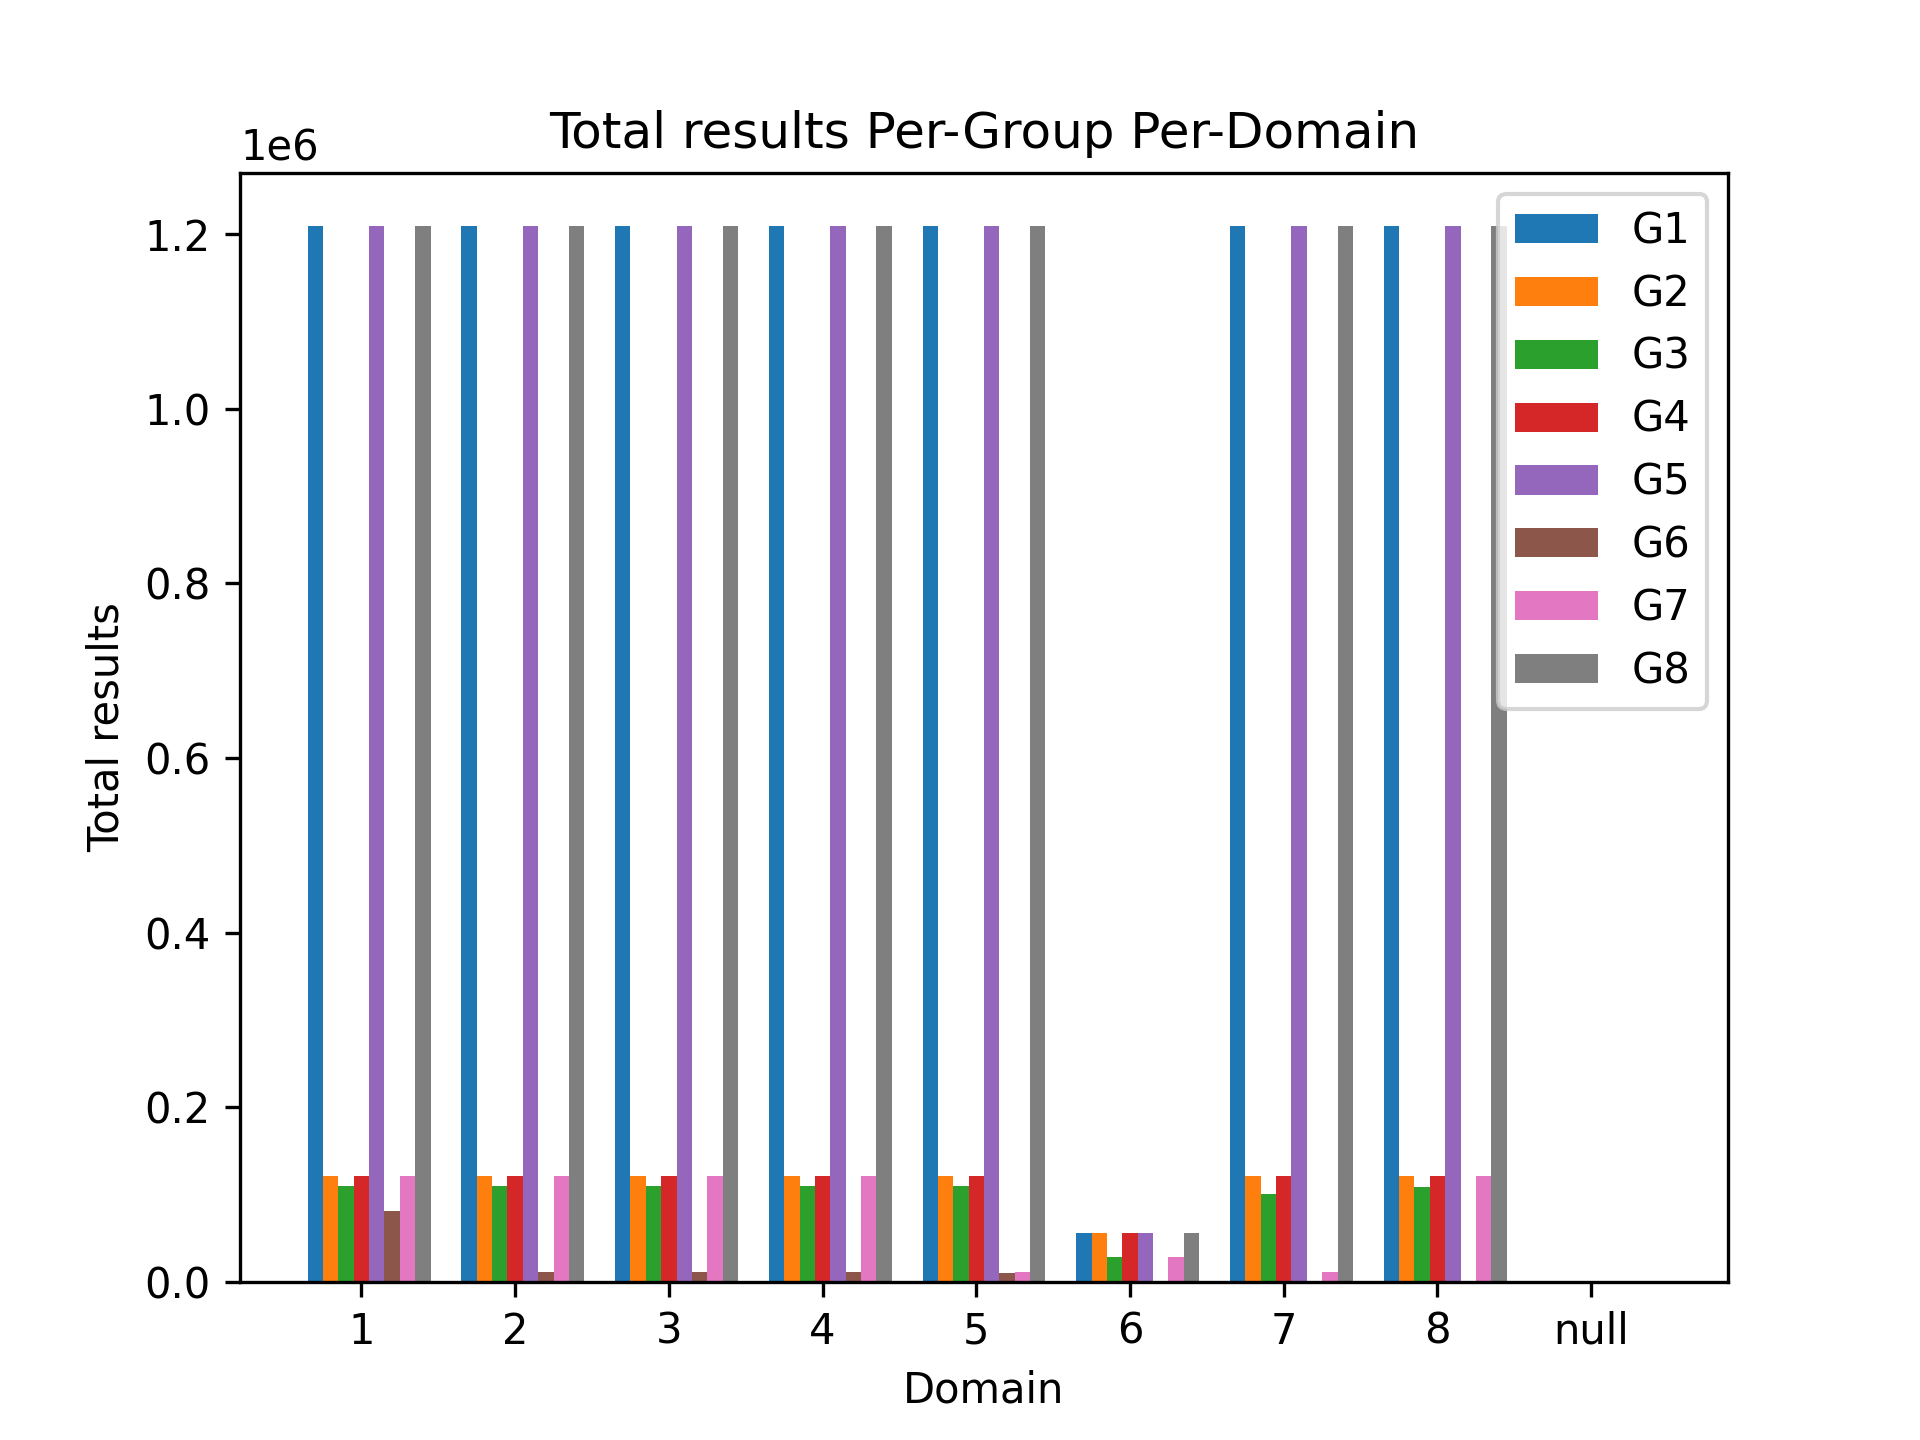
\includegraphics[width=0.9\paperwidth]{figures/group_domain_result_counts.png}
    }
    \caption{Total number of results per-group per-domain.}
    \label{fig:totals}
\end{figure}


\begin{equation*}
    \text{Average Recovery Rate} = \frac{\sum_i D^\text{score}_i}{i}
\end{equation*}

Bars in the visualizations below for groups with fewer datapoints should be considered to have a higher degree of error compared to groups with more datapoints. However, for all groups besides group 6, there are hundreds of thousands of datapoints per-domain, so these results should also be considered stable. We find that our agent is the top performer for domains 3, 6, and 7. For domains 4, 5, and 8, our agent is generally competitive with other top-performing agents. Our agent underperforms on domains 1 and 2.

\FloatBarrier

\subsection{Domain 1}
\makebox[\textwidth][c]{
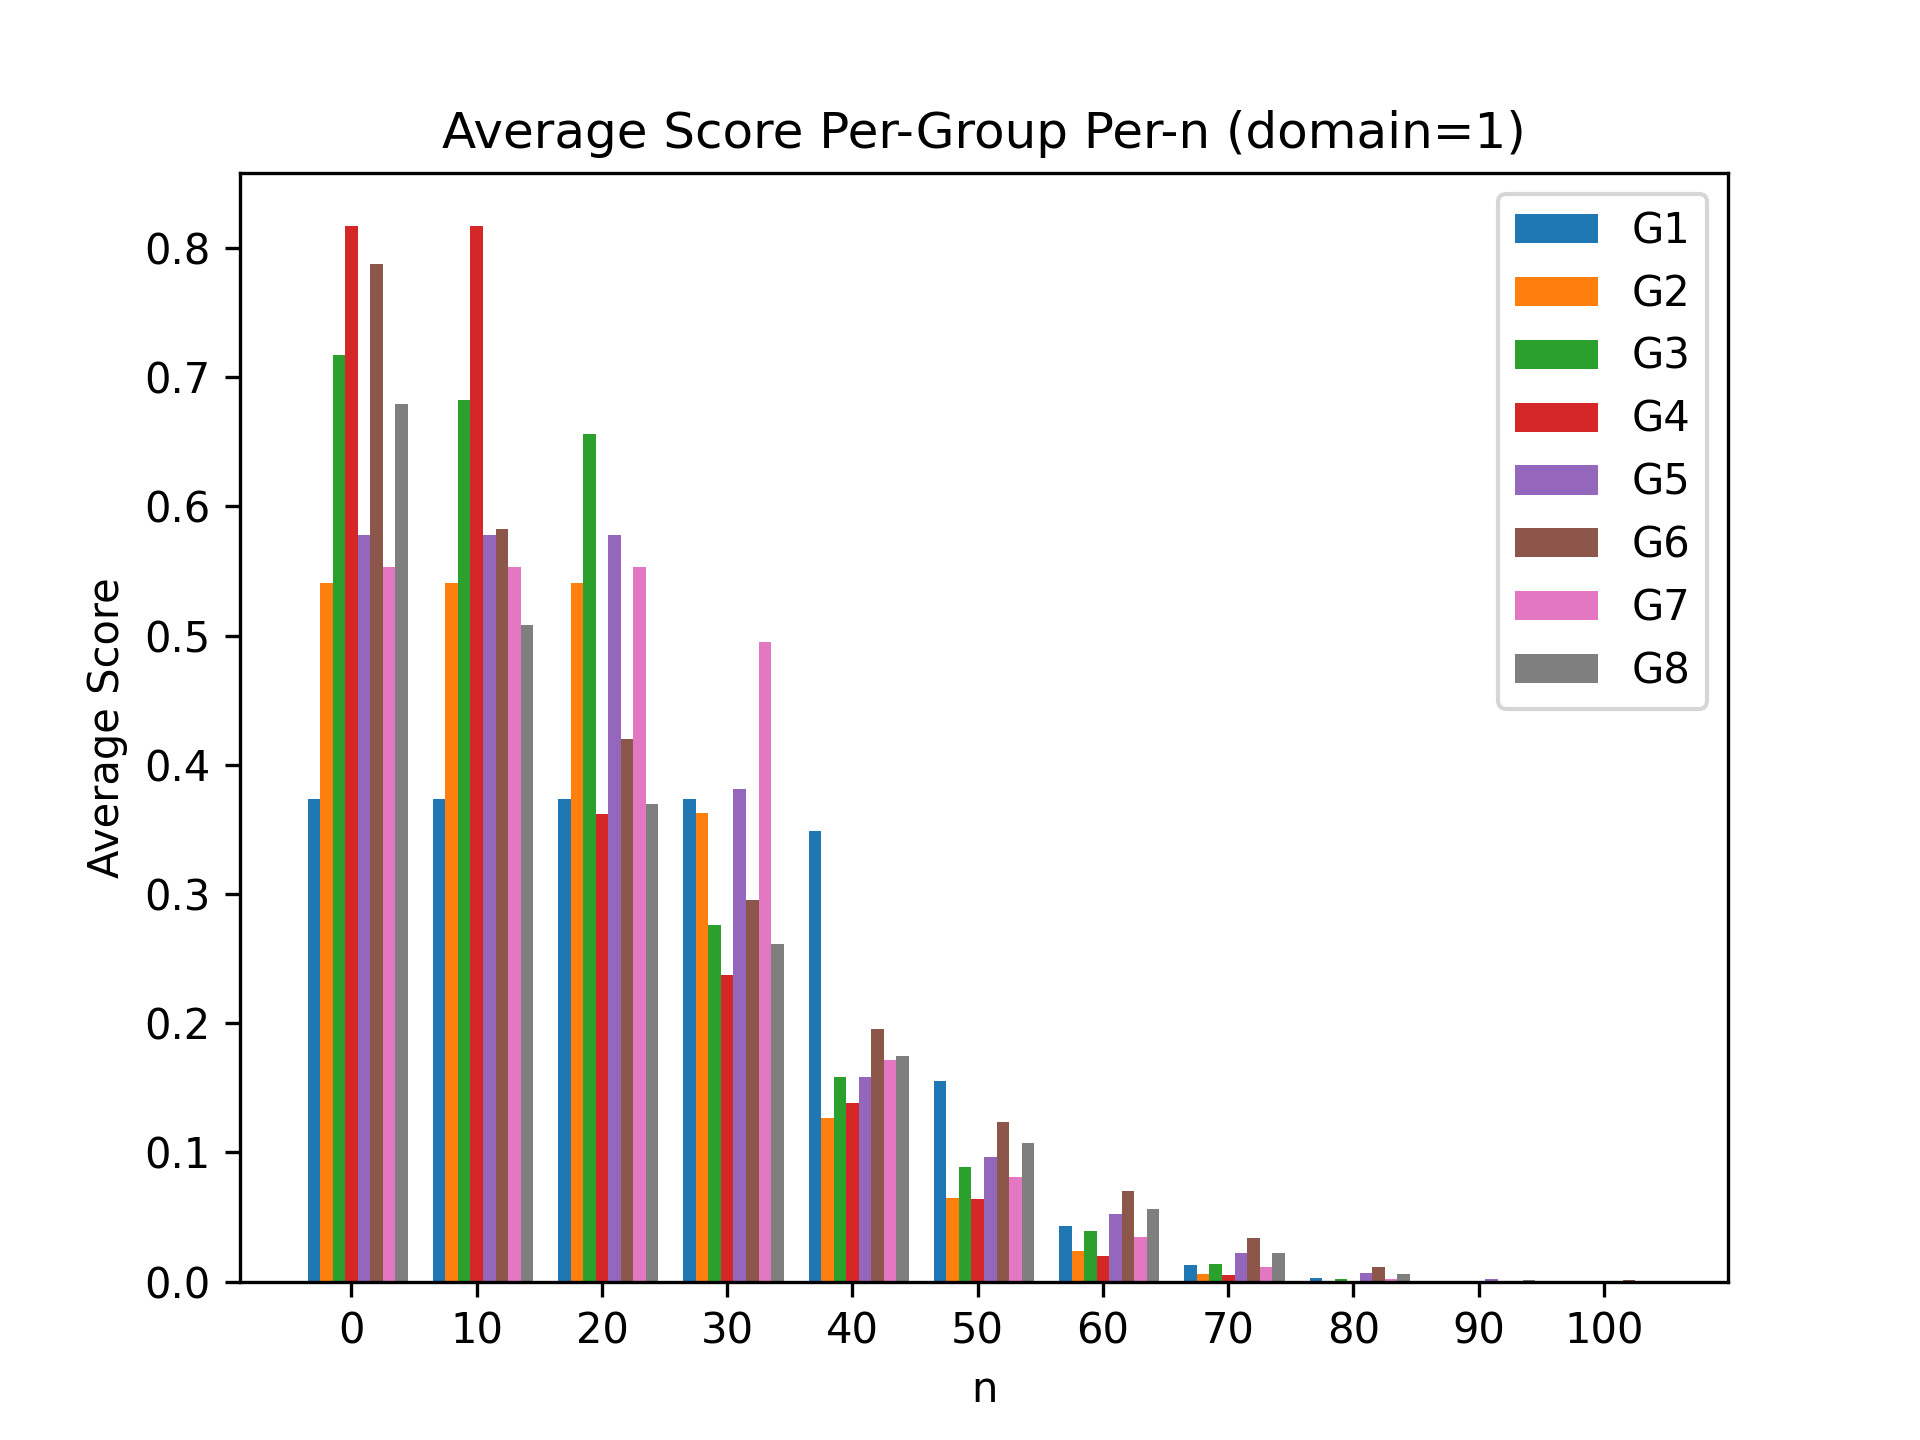
\includegraphics[width=0.9\paperwidth]{figures/domain_1.png}
}

For domain 1 (random characters), we find that our agent is generally competitive at higher values of $n$, but underperforms other agents for lower values of $n$. This is likely due to lack of support for truncation of long messages/partial recovery, as discussed in \Cref{future}.

\subsection{Domain 2}
\makebox[\textwidth][c]{
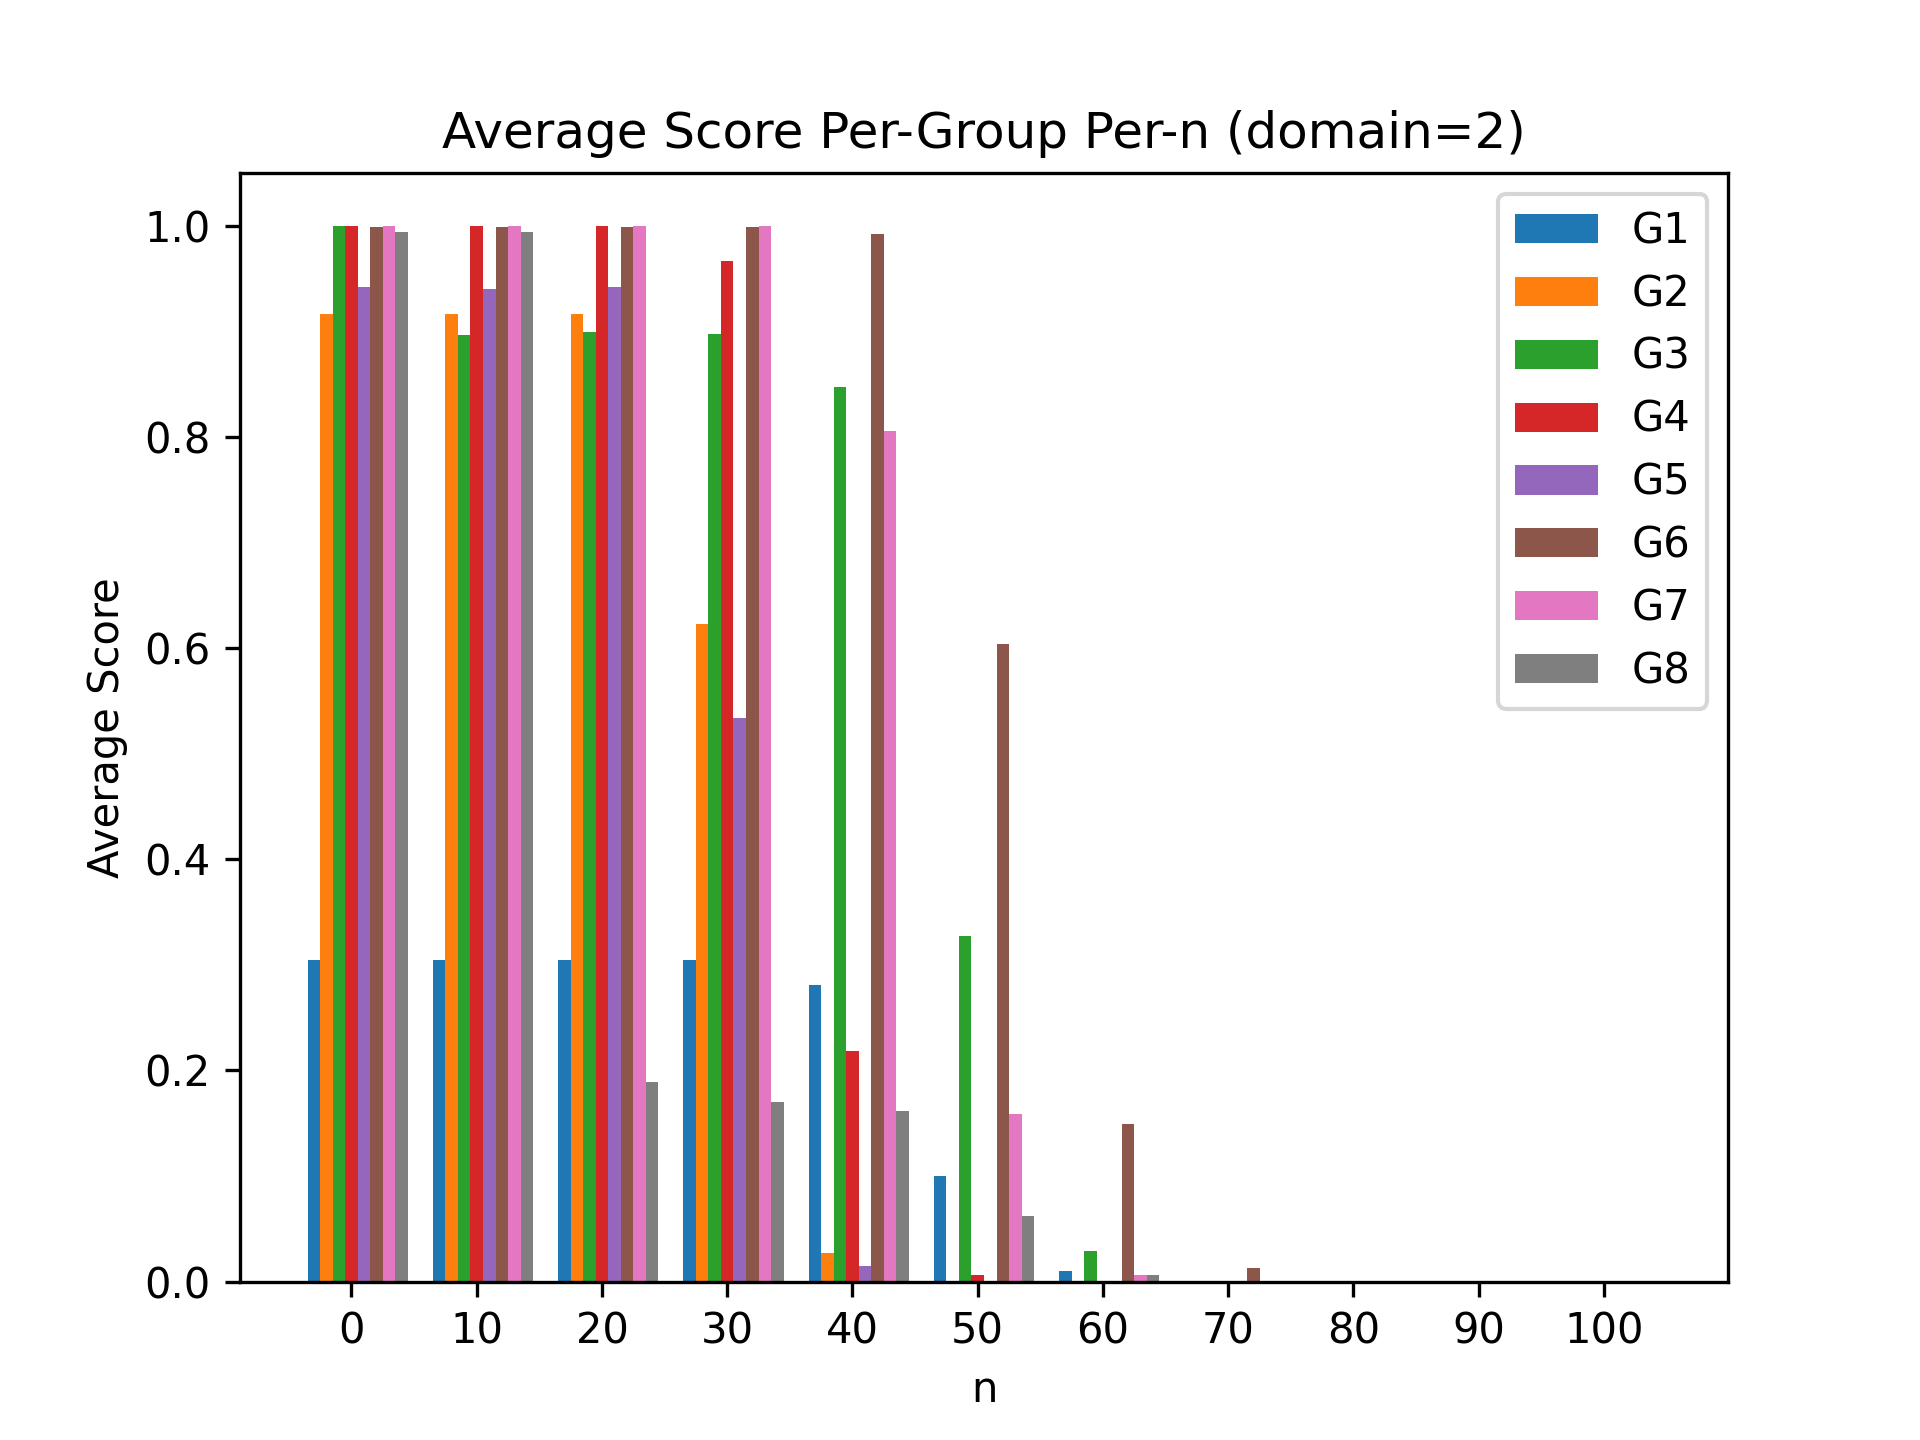
\includegraphics[width=0.9\paperwidth]{figures/domain_2.png}
}

For domain 2 (flights), our agent is competitive at $n=0, 10$, but has a sharp decrease in effectiveness at $n=20$. This domain is the one on which our agent underperforms by the largest margin. We investigated the reason for this and found that our codec for dates was failing to encode months/days with leading 0's. Fixing this trivial bug improved our agent's performance substantially, as shown below.

\makebox[\textwidth][c]{
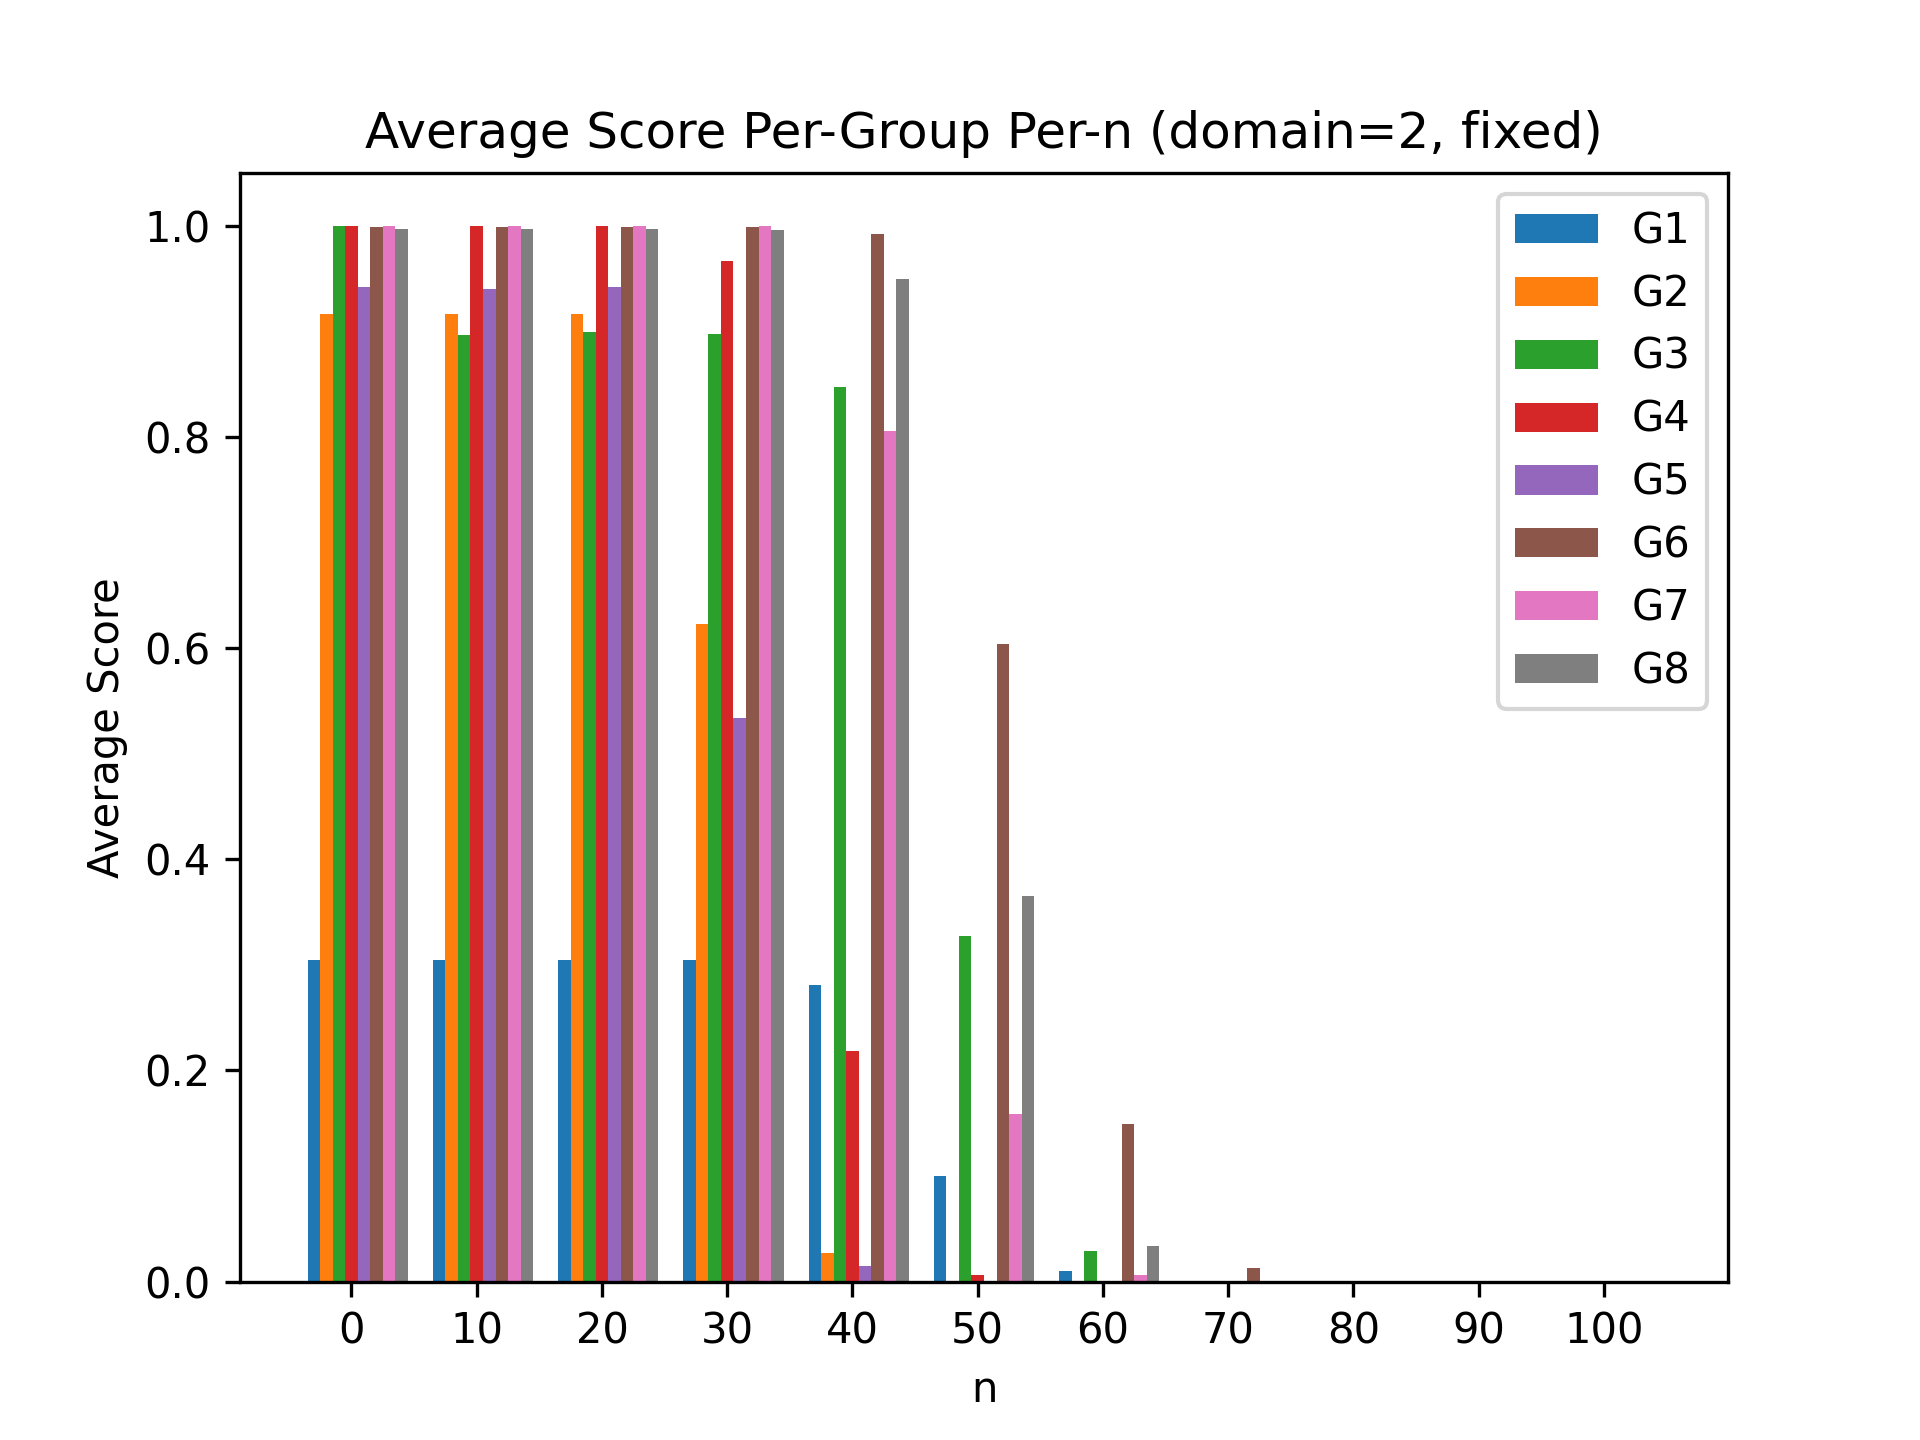
\includegraphics[width=0.9\paperwidth]{figures/domain_2_fixed.png}
}

As shown by the above figure, our agent is now one of the top-performing for domain 2 with the fix applied. We attribute this high performance to our compact message-to-bits representation of the flight domain, discussed in detail in \Cref{domains}.

\subsection{Domain 3}
\makebox[\textwidth][c]{
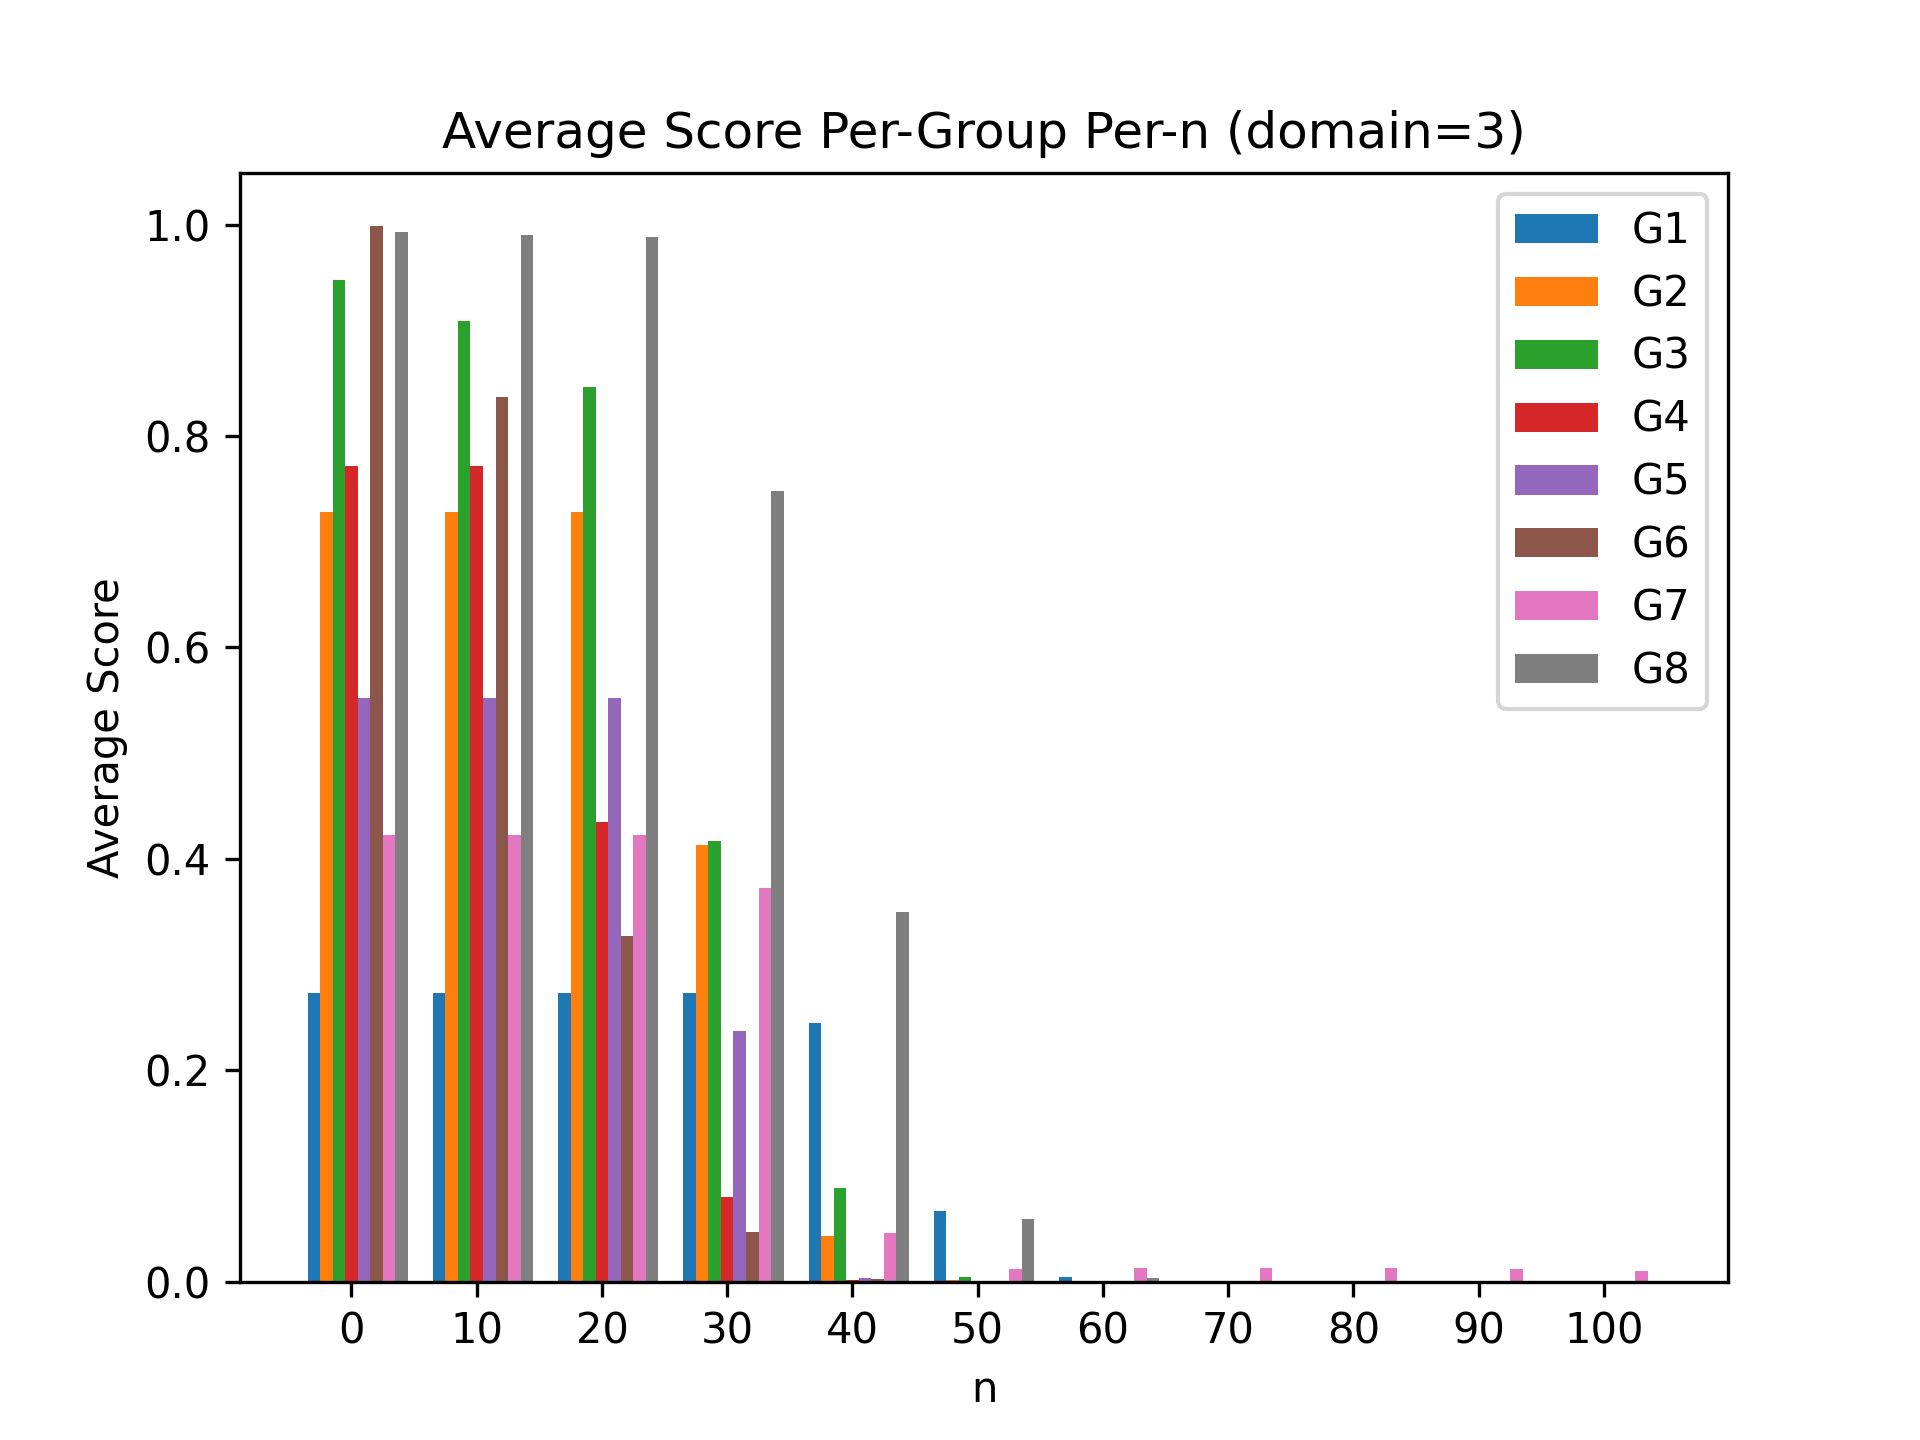
\includegraphics[width=0.9\paperwidth]{figures/domain_3.png}
}
For domain 3 (passwords), we are surprised to find that our agent is the clear standout winner. We attribute this performance to our compact message-to-bits encoding for this domain, discussed in detail in \Cref{domains}.

\subsection{Domain 4 \& 5}
\makebox[\textwidth][c]{
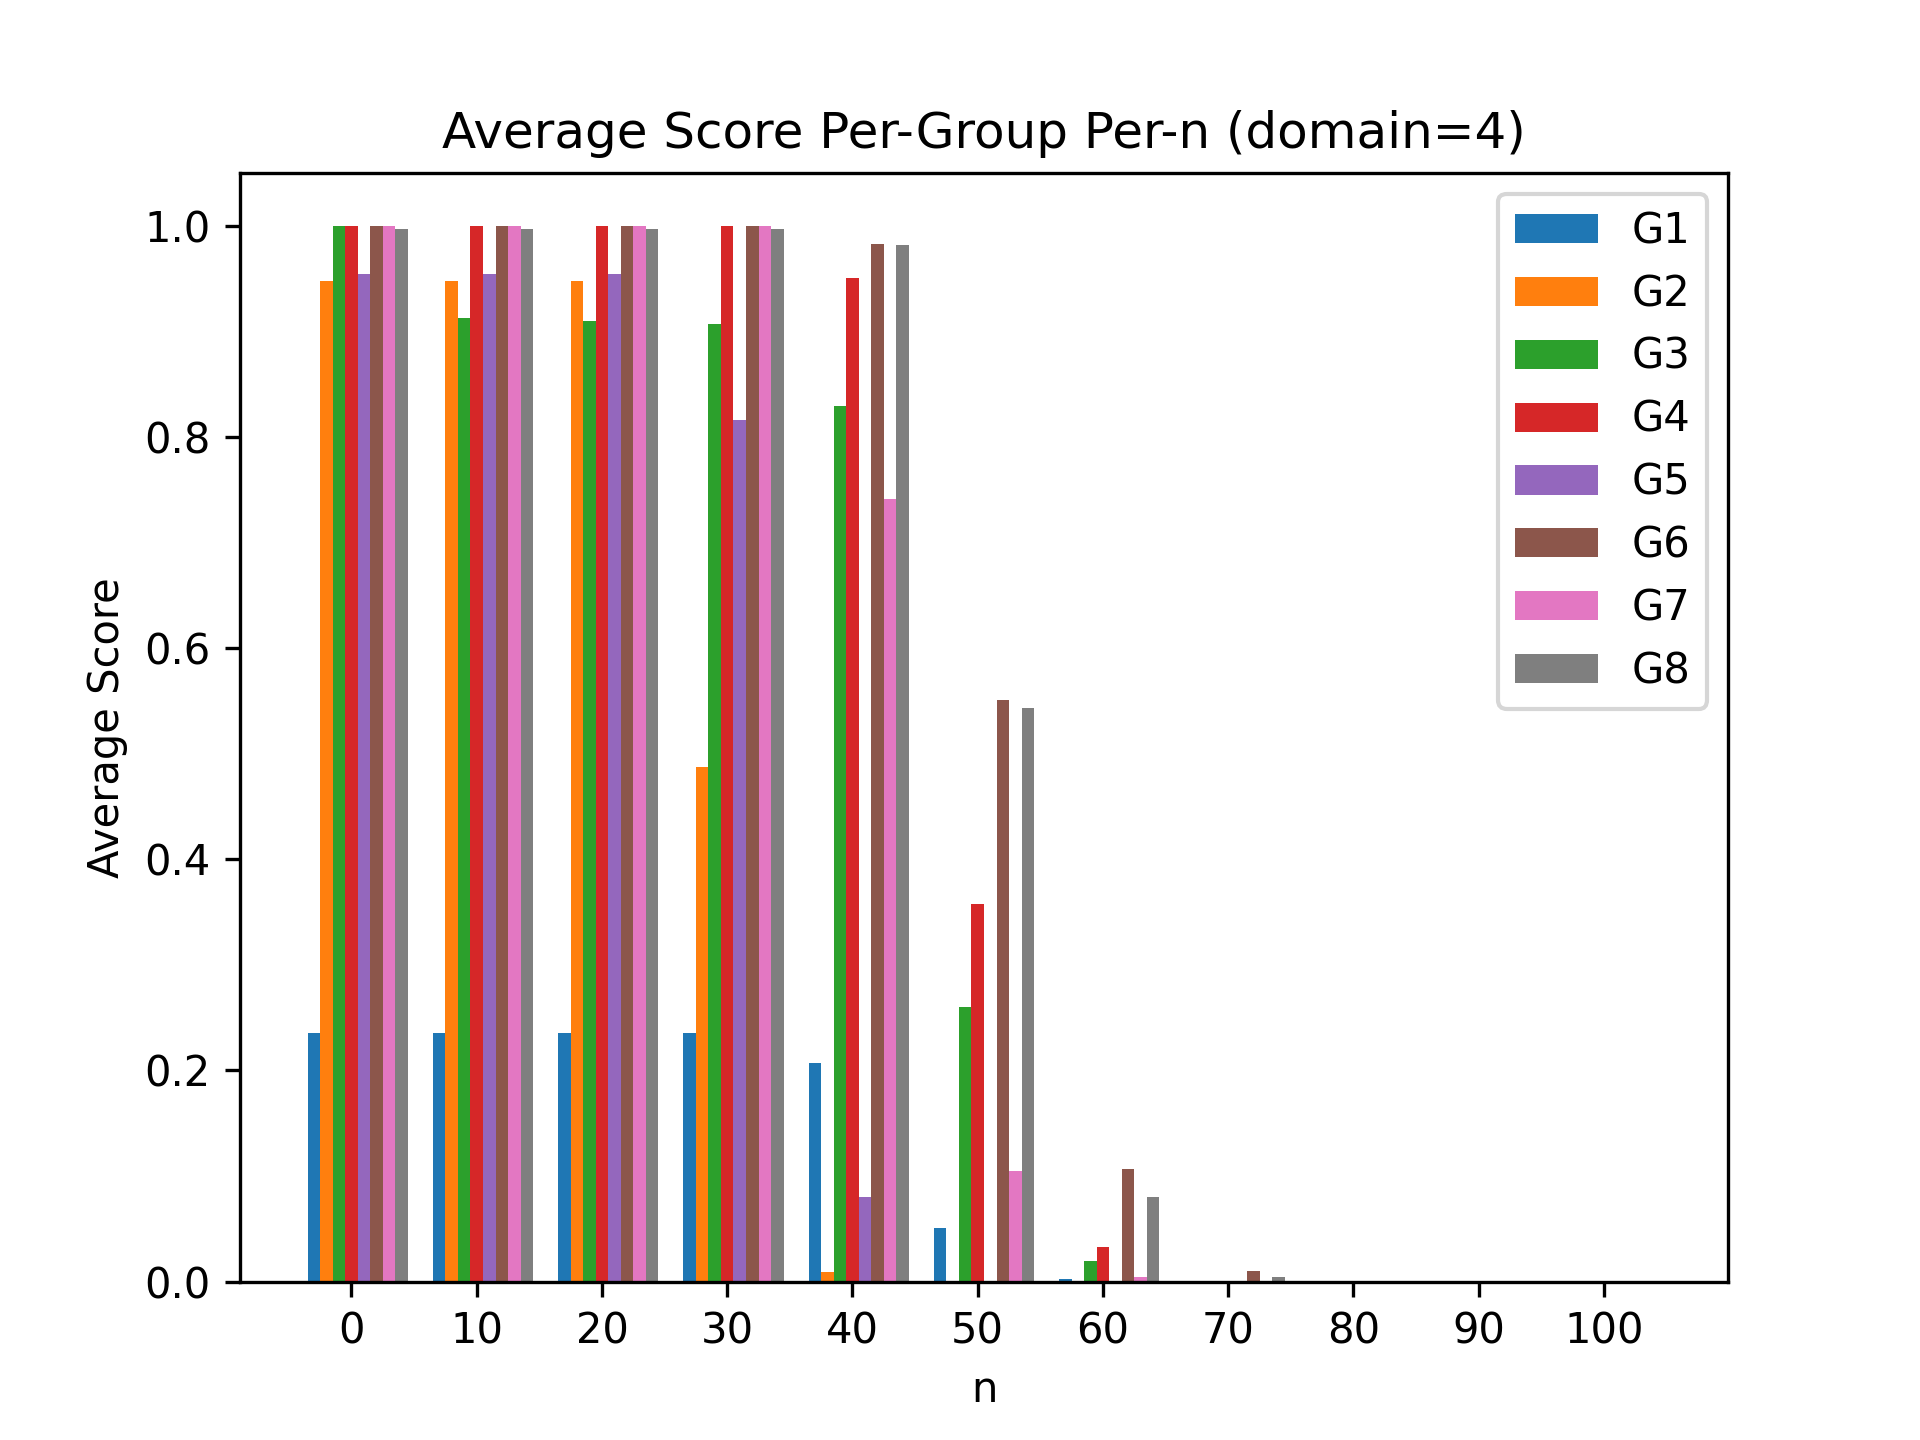
\includegraphics[width=0.45\paperwidth]{figures/domain_4.png}
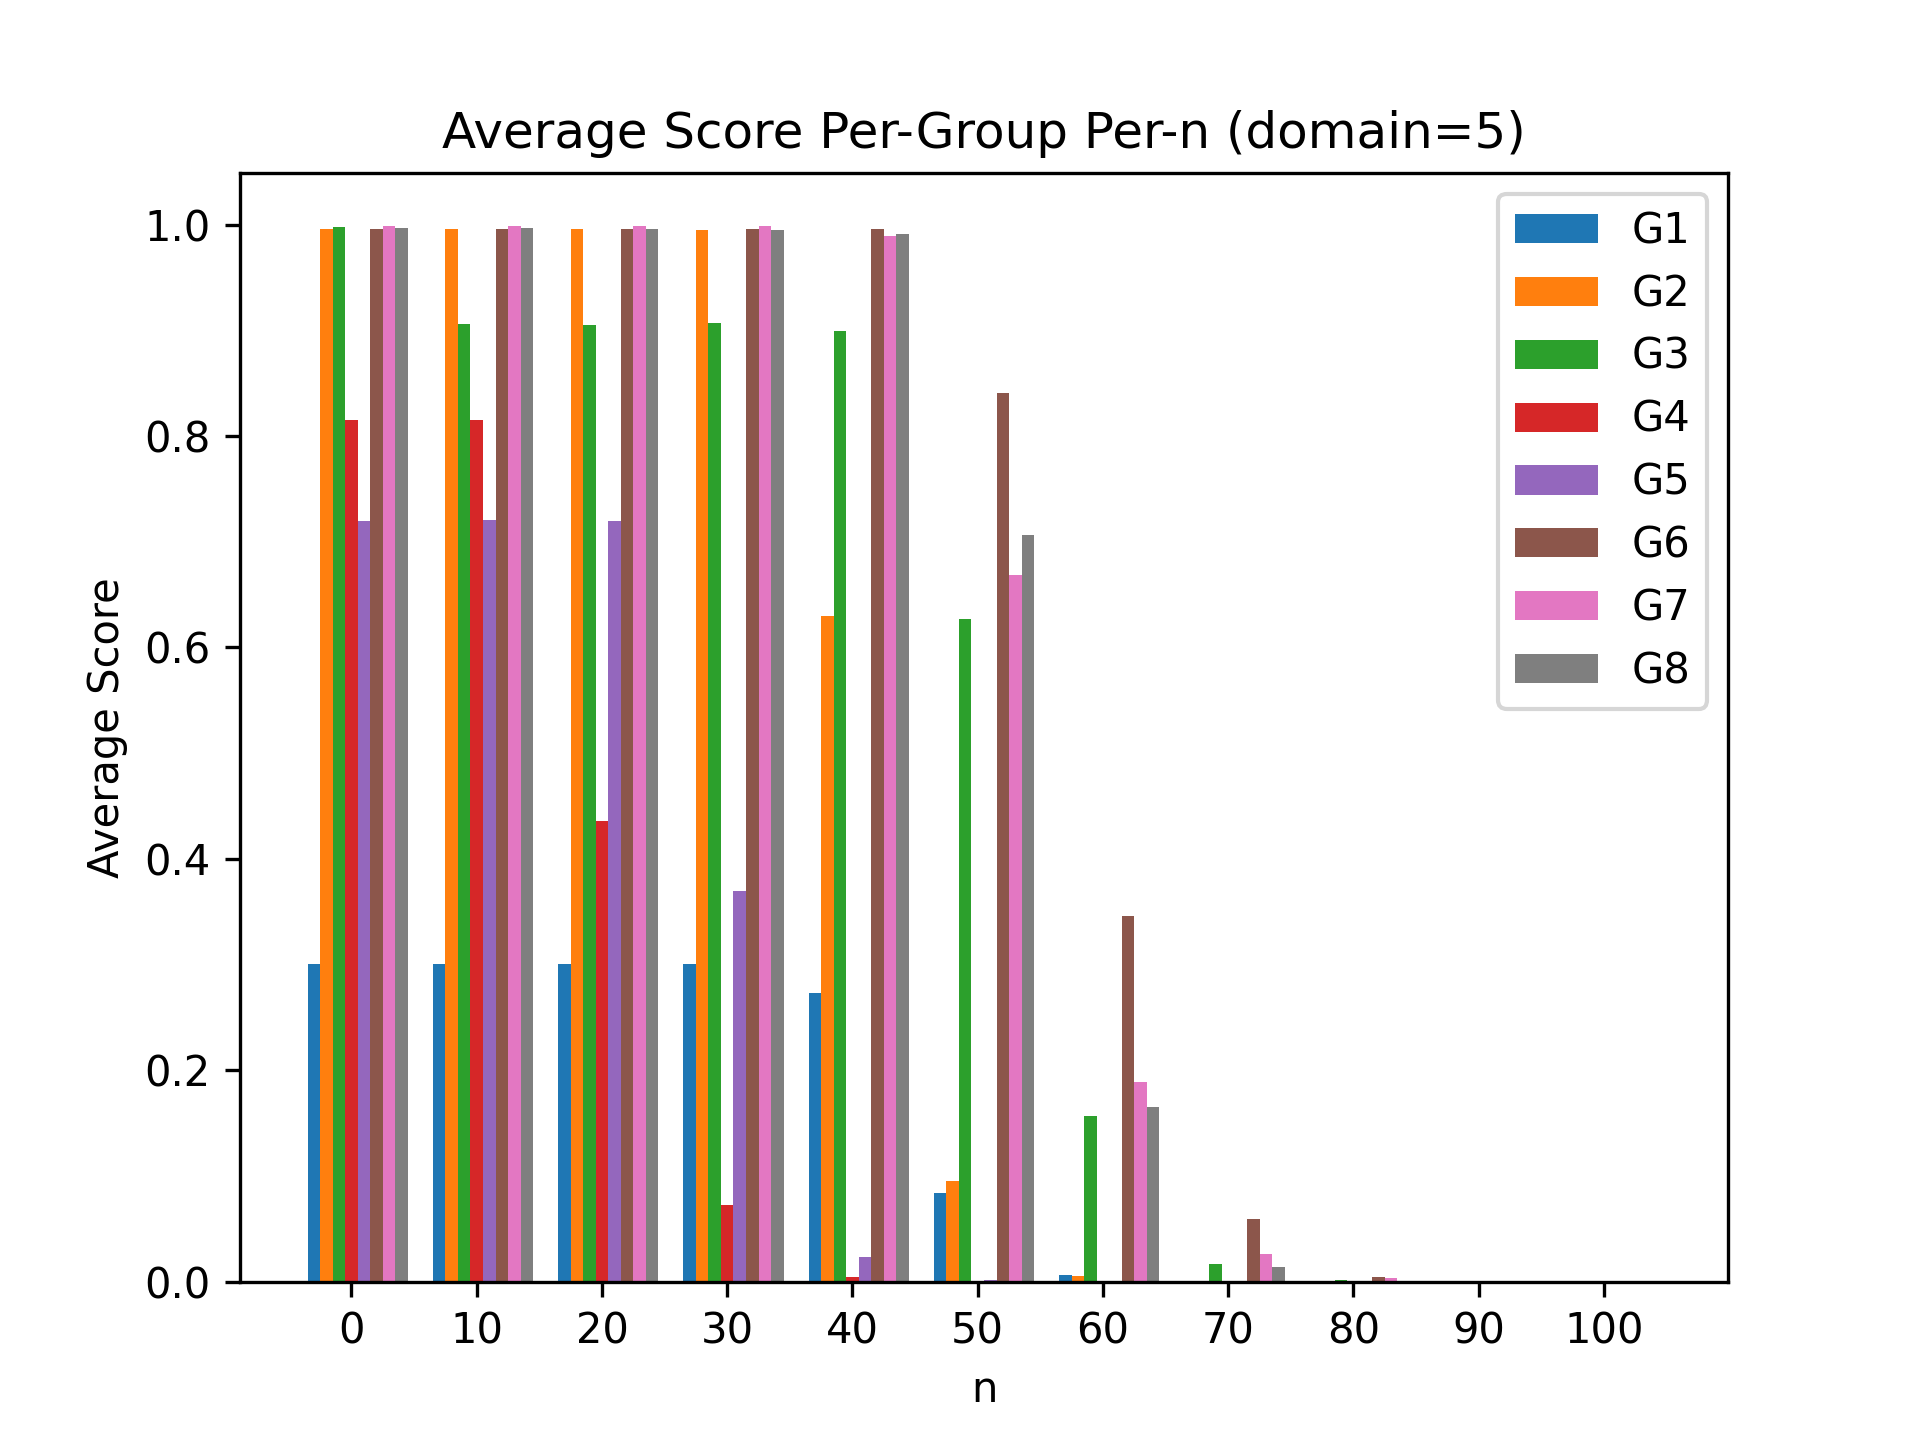
\includegraphics[width=0.45\paperwidth]{figures/domain_5.png}
}

For domains 4 (coordinates) and 5 (addresses), our agent is among the top performing. In domain 4, our agent is basically tied with Agent 6 on higher values of $n$. In domain 5, Agent 6 has a slight lead for higher value of $n$.

\subsection{Domain 6 \& 7}
\makebox[\textwidth][c]{
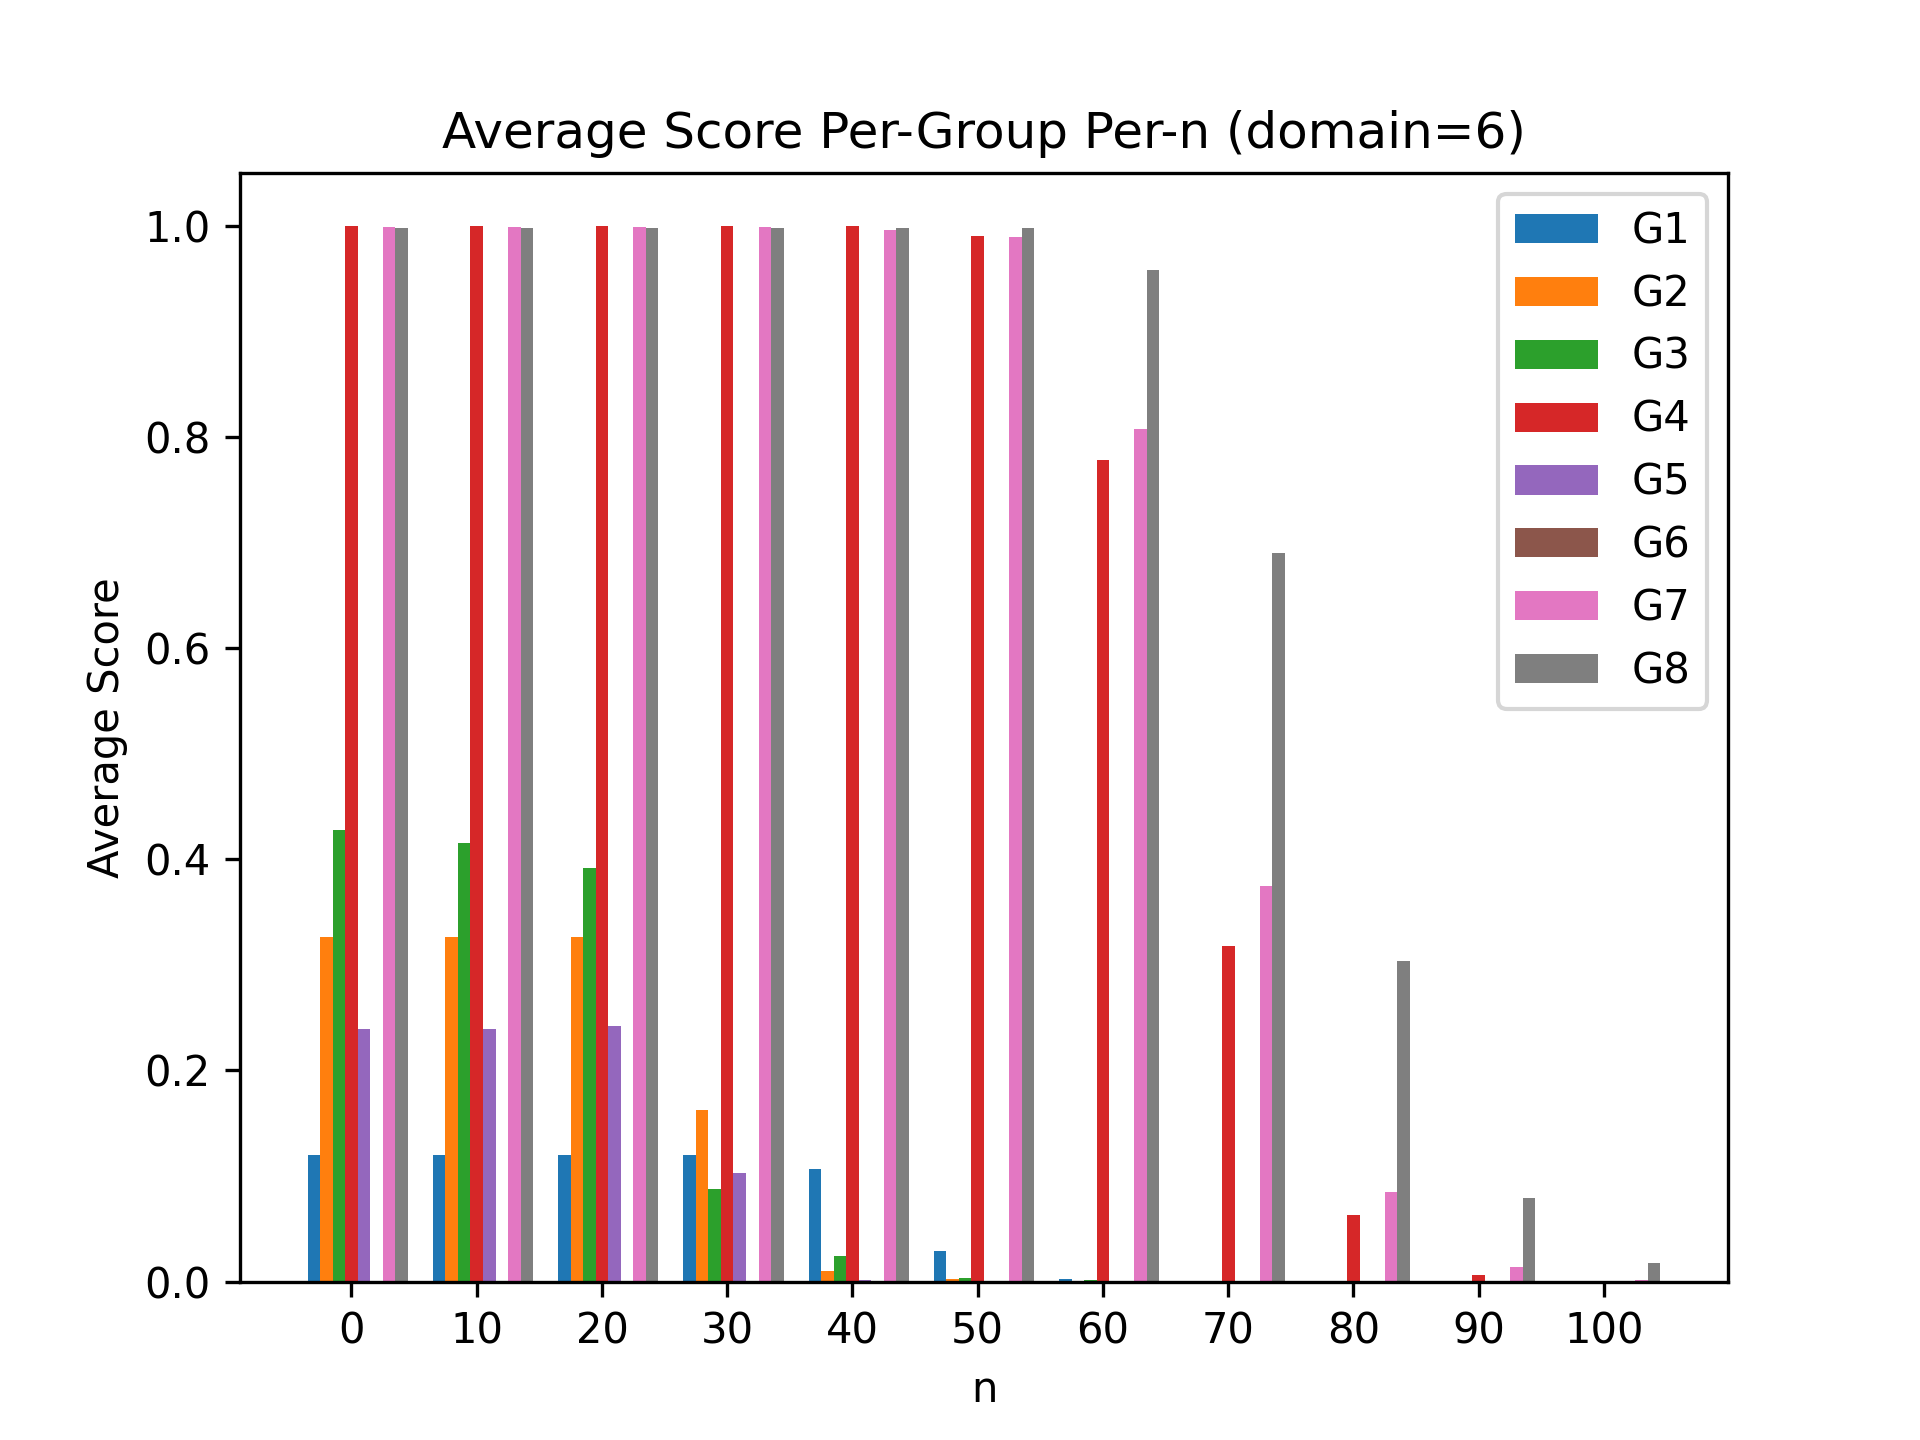
\includegraphics[width=0.45\paperwidth]{figures/domain_6.png}
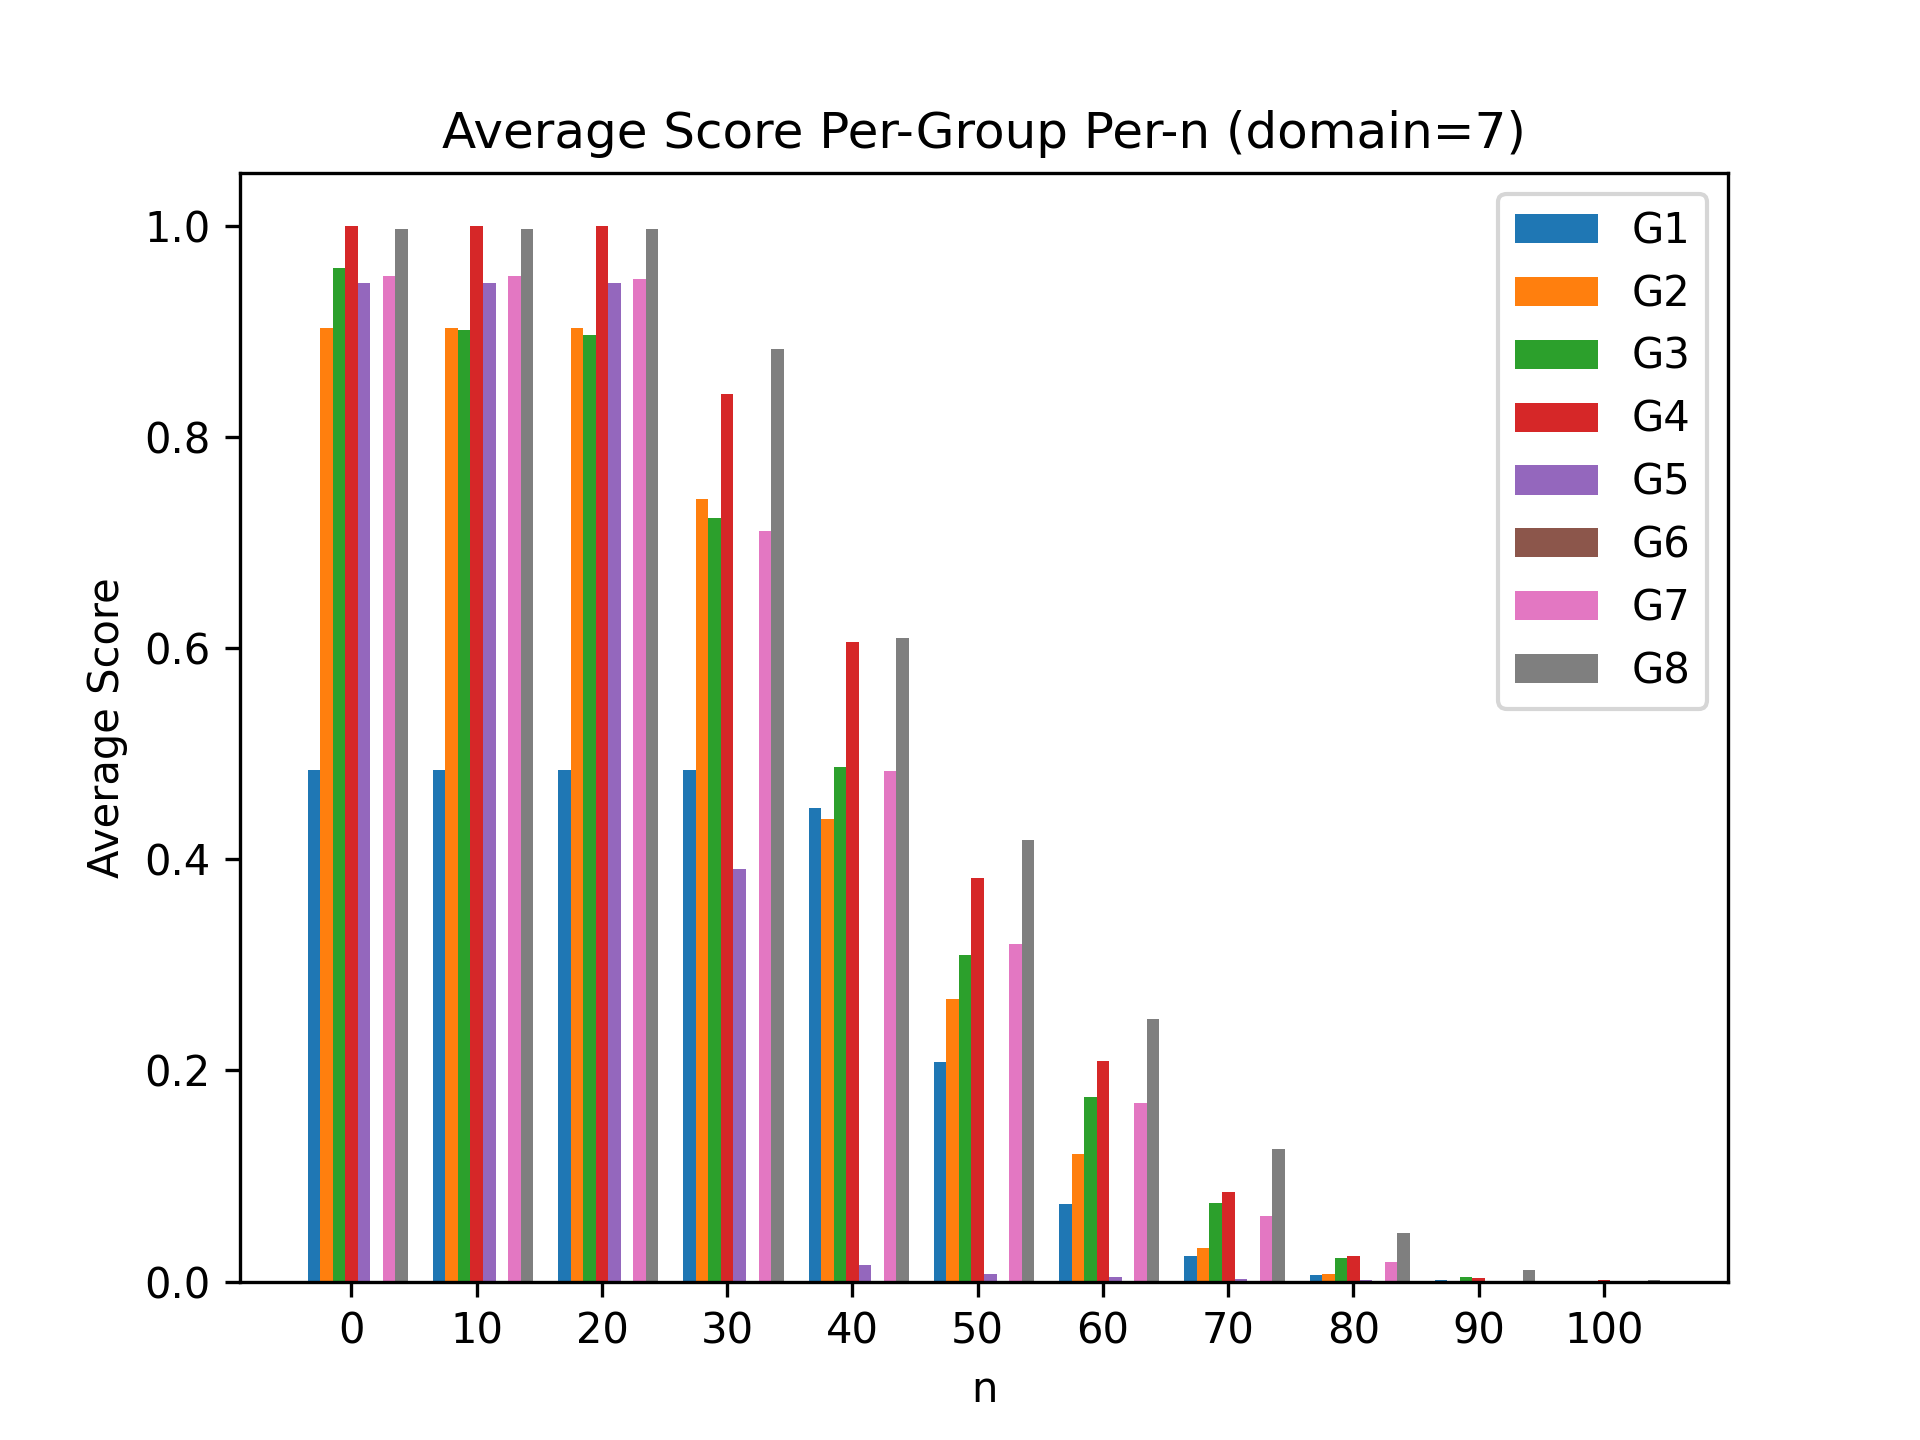
\includegraphics[width=0.45\paperwidth]{figures/domain_7.png}
}

Domains 6 (n-grams) and 7 (words) are both dictionary-based domains that are very easily represented using our \textbf{dictionary indexing} technique. As such, we achieve a very compact binary representation for the messages and are the best-performing group at high values of $n$. Domain 6, in particular is highly compact, which is why a substantial proportion of messages from that domain can survive to $> 70$ shuffles.

\subsection{Domain 8}
\makebox[\textwidth][c]{
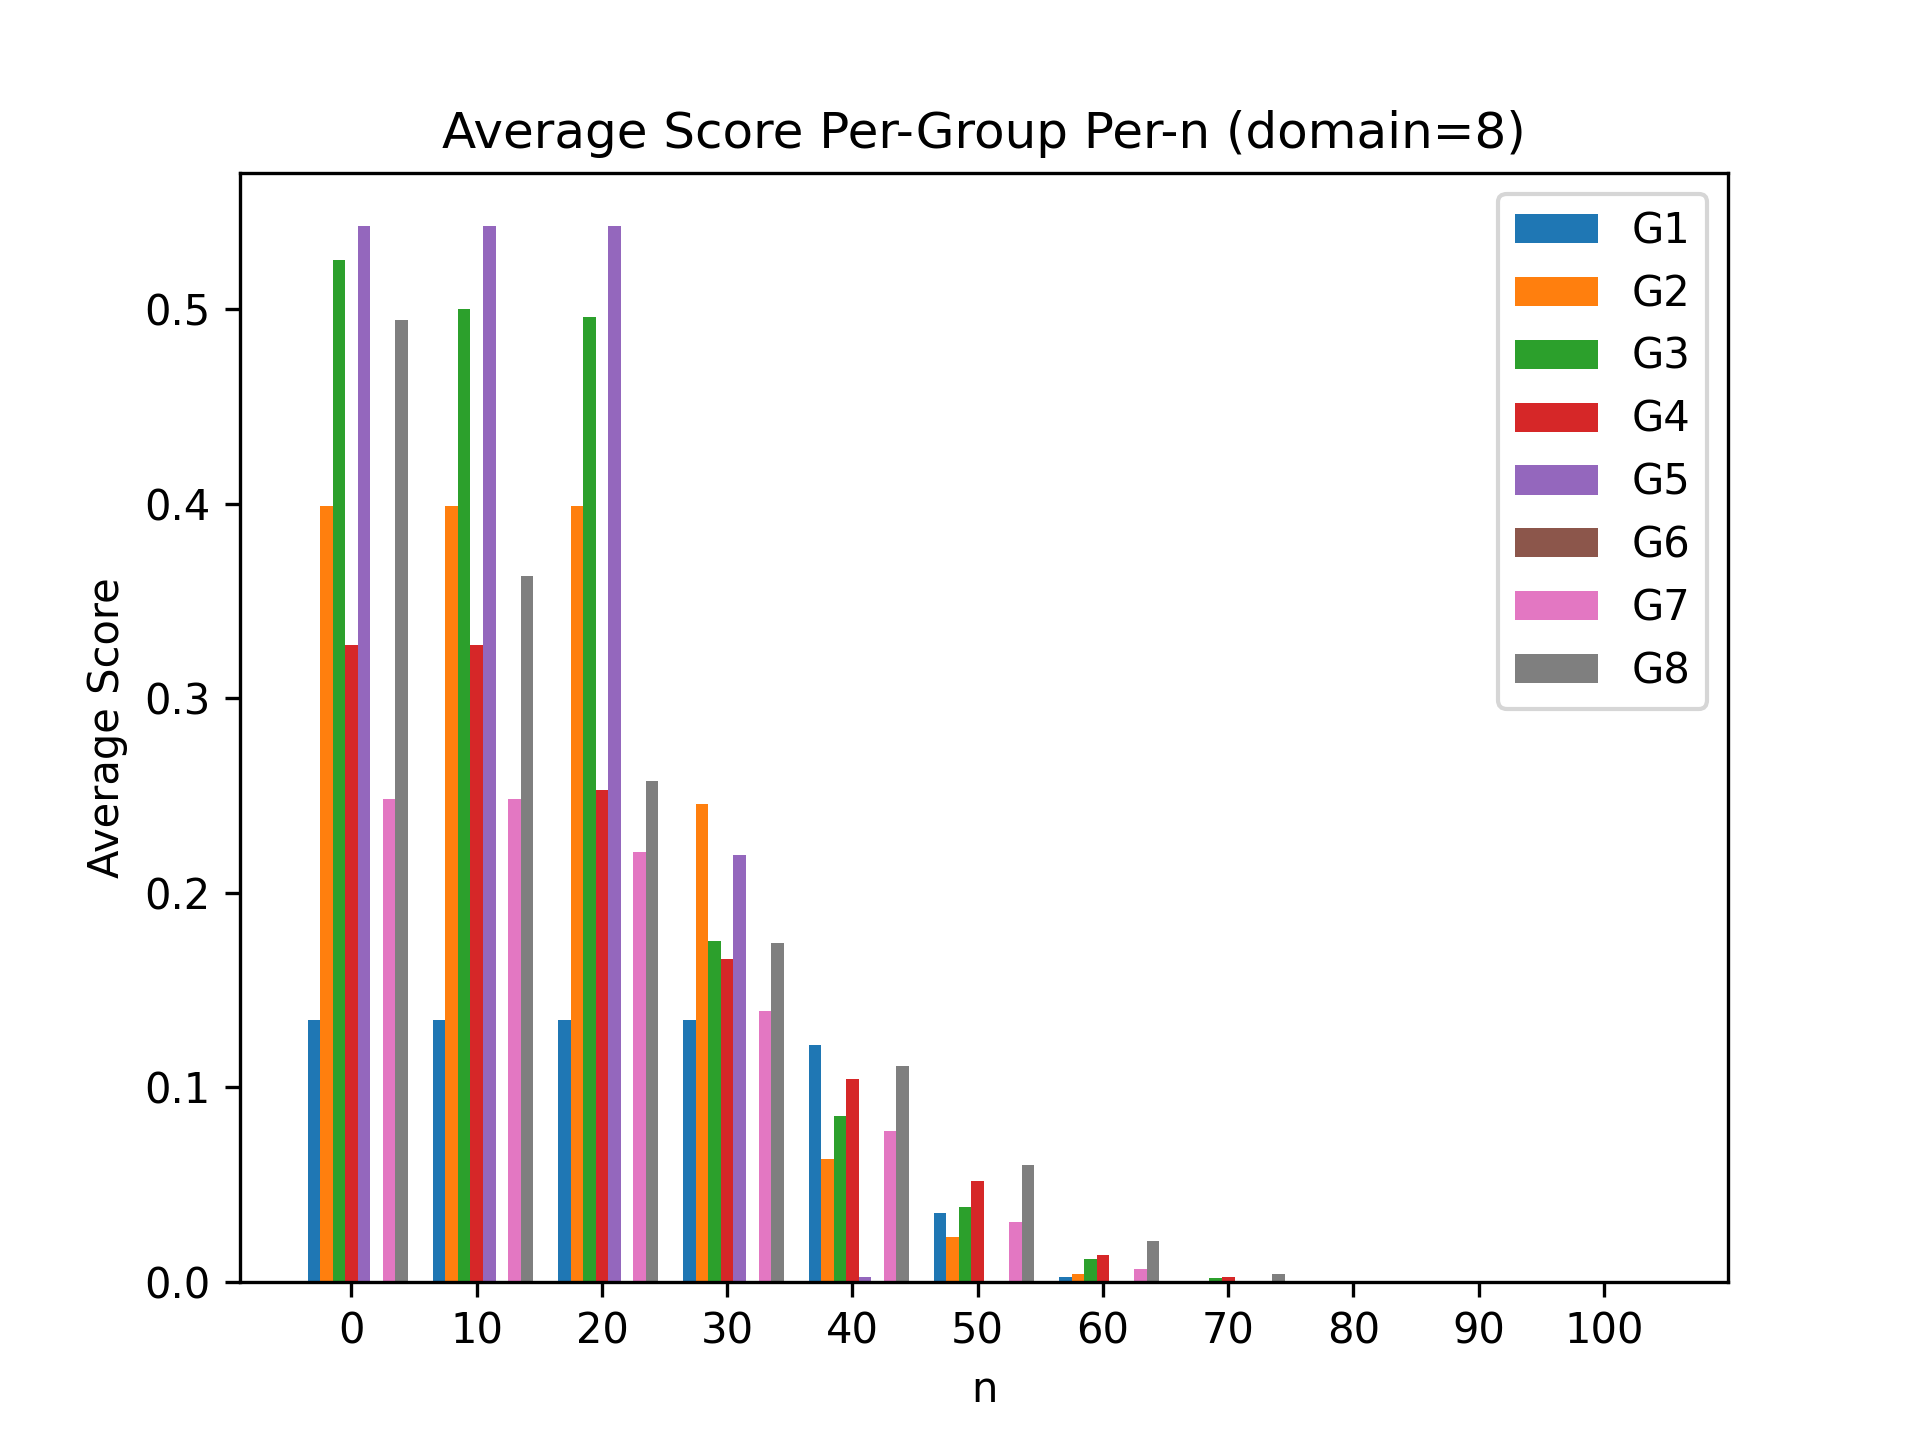
\includegraphics[width=0.9\paperwidth]{figures/domain_8.png}
}

For domain 8 (names and places), Our agent slightly underperforms other agents for low values of $n$. We attribute this to lack of support for truncation of long messages/partial recovery. As the generator for this domain supports arbitrary length messages, there are some messages that the encoder simply rejects for being too long. A resolution for this is discussed in \Cref{future}.

\subsection{NULL Domain}
\makebox[\textwidth][c]{
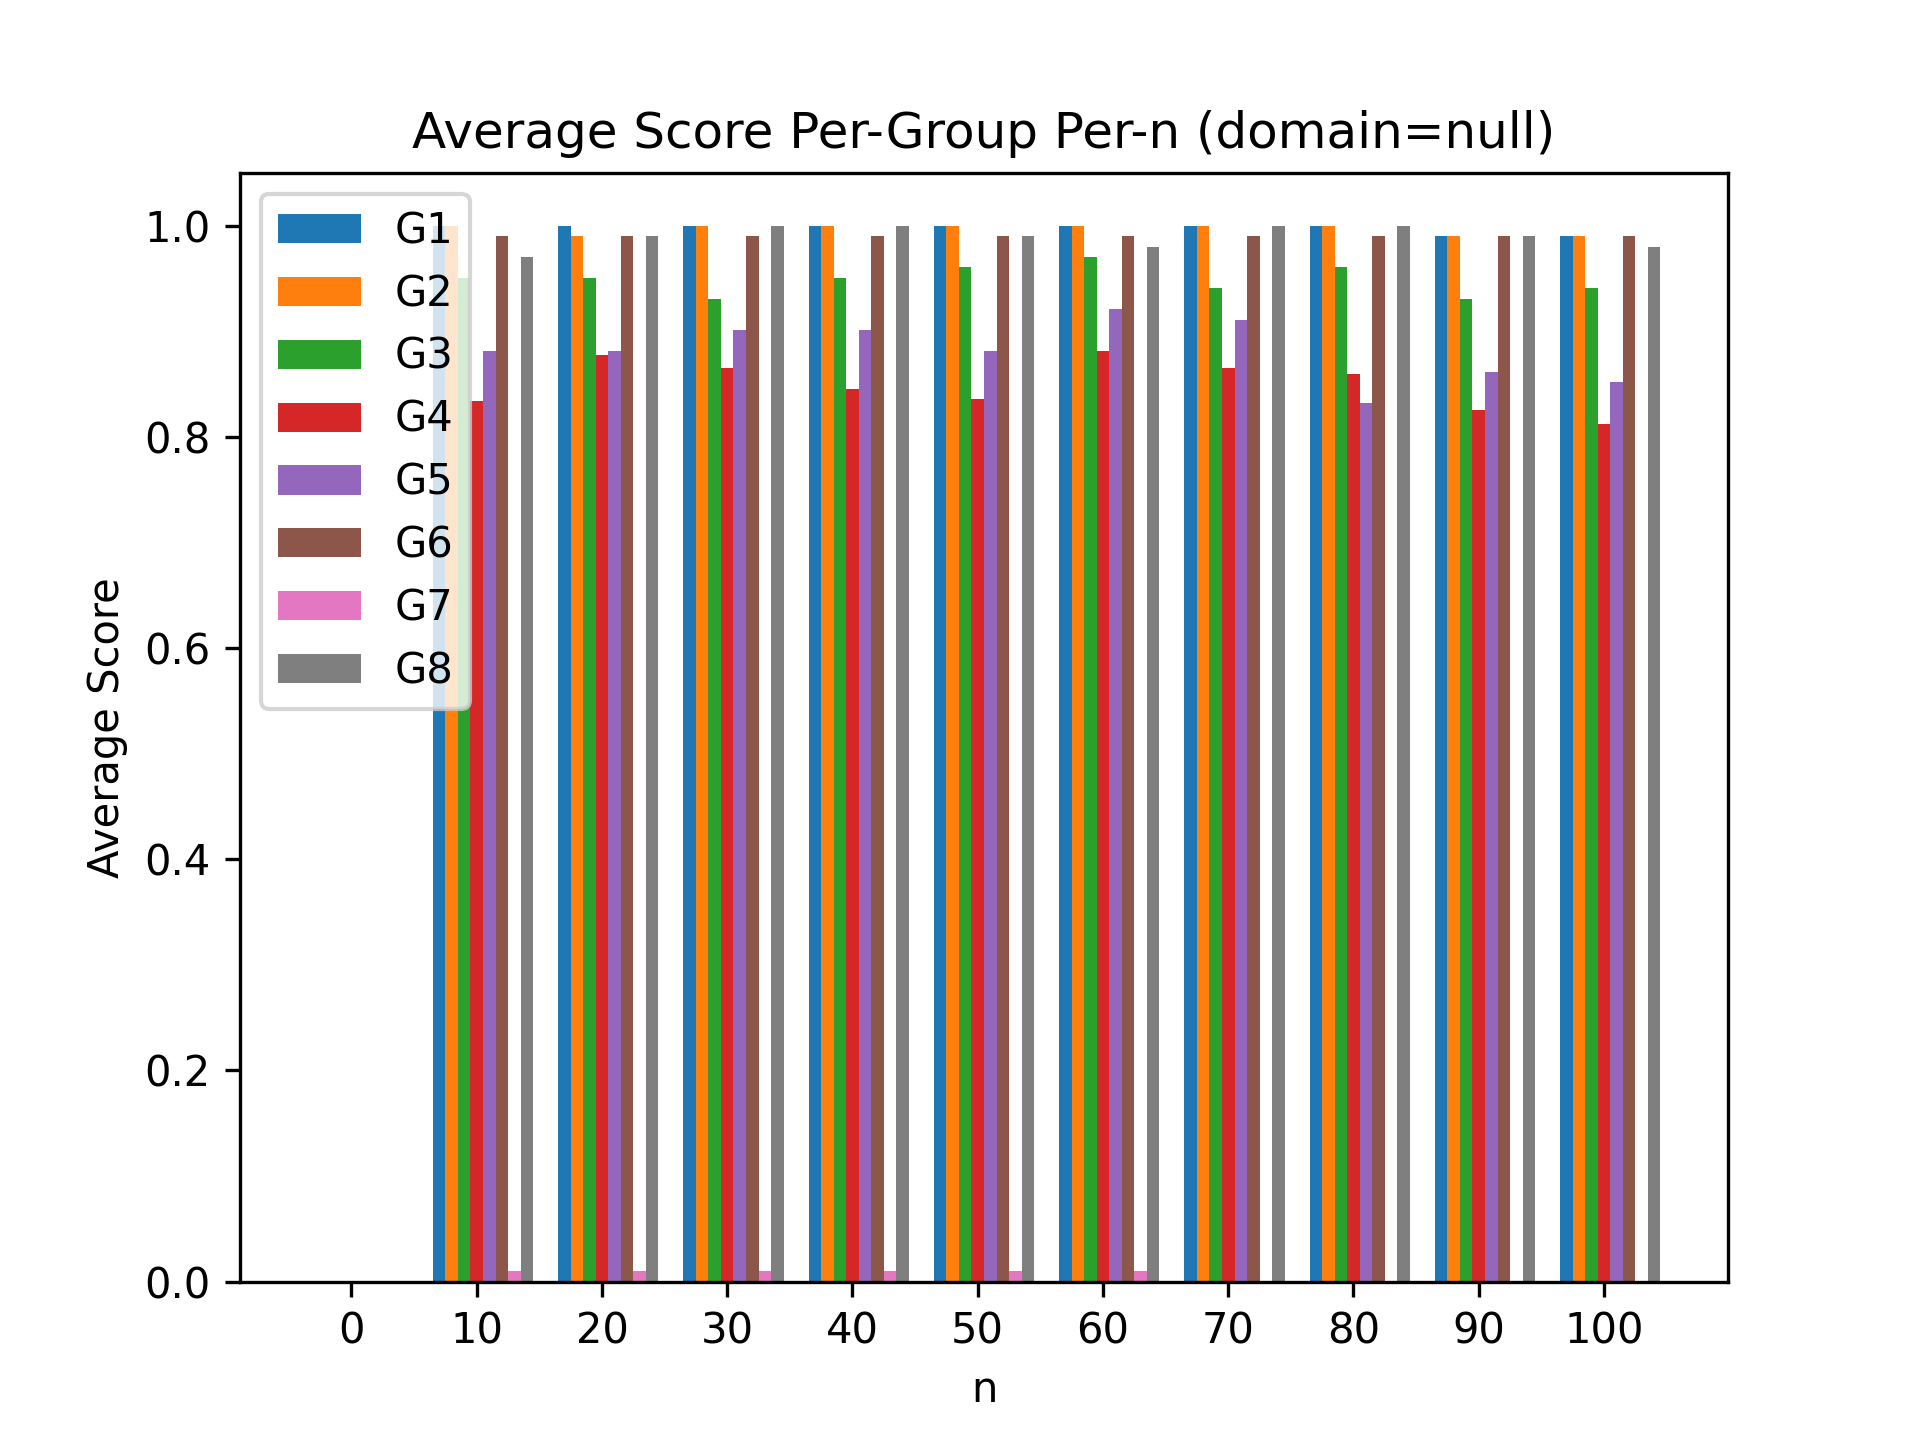
\includegraphics[width=0.9\paperwidth]{figures/domain_null.png}
}

Most agents perform well on the NULL domain. We find that our agent is among the top performers for rejecting NULL decks across values of $n$. We attribute this high performance to our long checksum (10 bits), which makes the probability of interpreting a random deck as a valid message low.



\section{Conclusion}

Our agent employs an index-based bits-to-cards encoding and a variety of domain-specific message-to-bits encoders. We are generally satisfied with the performance of our agent in the tournament.

\subsection{Failed Recovery at $n=0$} \label{n_0}
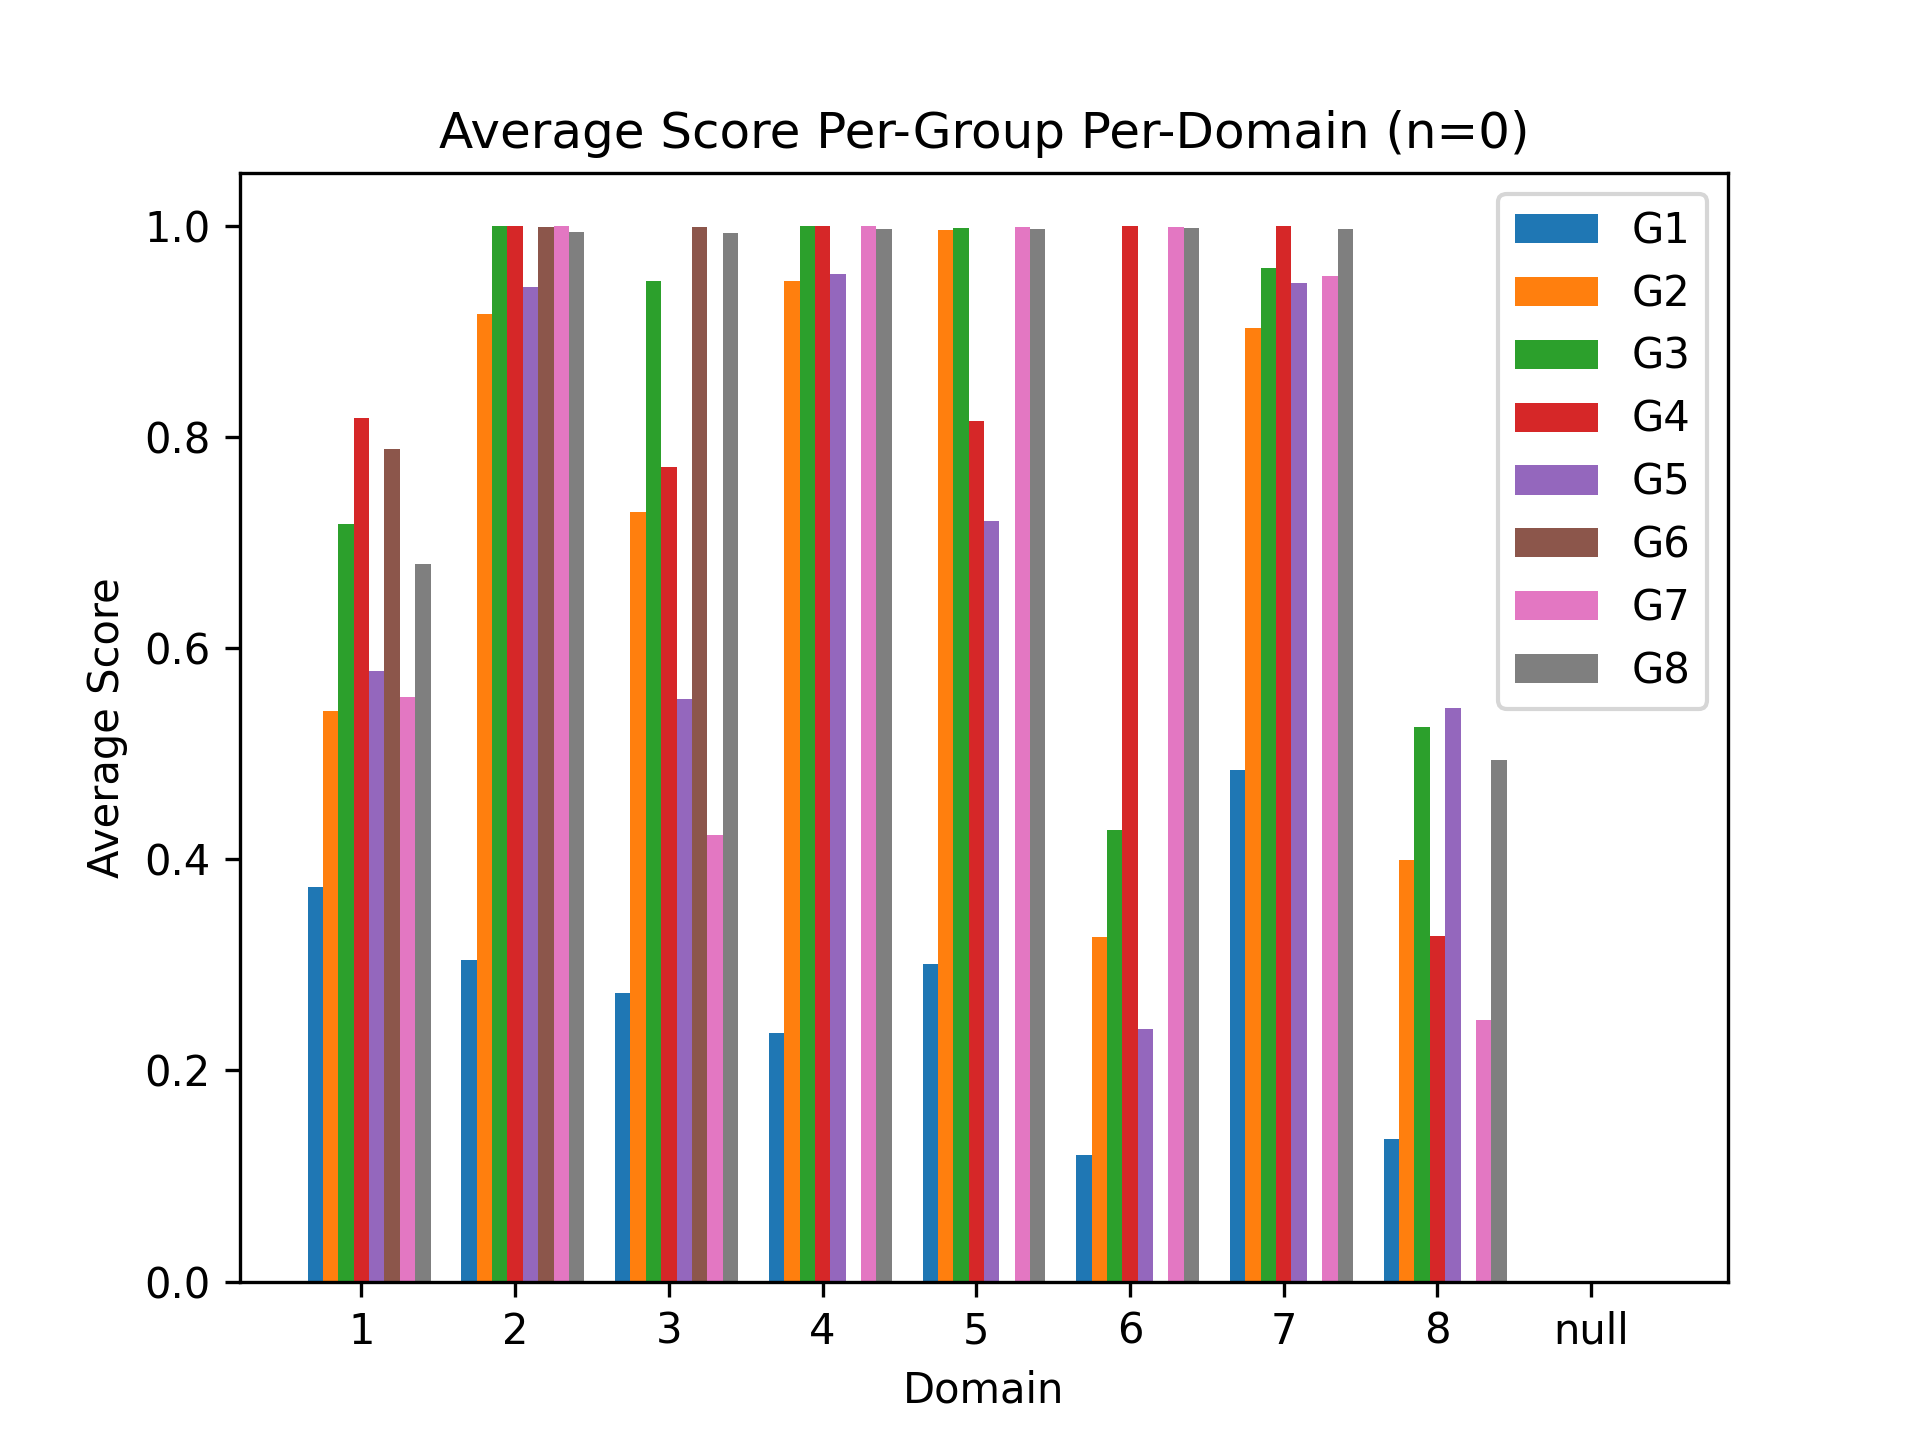
\includegraphics[width=\textwidth]{figures/n_0.png}

The plot above shows recovery rates for $n=0$, i.e. no shuffles, across all domains. Our recovery rate is not perfect for some domains. This is caused by a combination of two factors: long messages and mistaken recovery. The dominant factor in why our recovery rate is not perfect for $n=0$ on domains 1 and 8 is message length: for messages that are too long to encode in the deck, we do not attempt to shorten the message and perform a partial decode. This effect is most pronounced on domains 1 and 8 because the generators for 1 and 8 have configurable lengths, allowing arbitrarily long messages to be generated.

For cases of mistaken recovery, we recover \textit{the wrong message} despite there being no shuffles. This is caused by checksum collisions between encoding domains in our variable-card encoding scheme. Since we do not know $c$, the number of cards used to encode a message in the deck, we attempt increasing values of $c$ until we find a message that passes the checksum. It is possible that at some incorrect, lower value of $c$, a different domain's message passes the checksum and is returned. This false positive rate can be lowered by increasing the number of checksum bits, which trades off against message survivability since, as discussed above, longer messages are more likely to be corrupted by fewer shuffles.

\subsection{Future Work} \label{future}
Our agent could perform significantly better if it supported partial recovery via truncated messages. As discussed in \Cref{n_0}, messages that are too long will fail to be encoded. A better strategy would be to remove tokens from the end of the message and attempt to re-encode until the message fits in the deck. We expect that applying this strategy would improve our agent's performance on longer messages in Domains 1 and 8.

Our agent does not support partial recovery for messages corrupted by shuffles. As discussed in class, partial recovery would require a break from the index-based bits-to-cards encoding scheme that most groups used. Using fewer cards results in significantly lower bit density per-card, making trading off between partial recovery and bit density difficult.

\subsection{Acknowledgements}
We would like to acknowledge Group 3 (Xiaozhou Shi, Rashel Rojas, Noah Silverstein) for the tip to use a single preceding 1 bit instead of a length byte to preserve leading zeros in the message body. This saved 7 bits in our message metadata, which allowed our encoding scheme to survive to higher shuffles than before.

\subsection{Summary of Contributions}
Jeff worked on the ``index''-based bits-to-cards encoding scheme, the metadata structure, and the custom domain encoders for tournament domains.


\end{document}